\documentclass[12pt,a4paper]{book}
\usepackage[bottom=2.5cm,top=3.5cm]{geometry}
%\usepackage{ngerman}
\usepackage[utf8]{inputenc}
\usepackage[T1]{fontenc}
\usepackage{graphicx}
\usepackage{colortbl}
\usepackage{ae}
\usepackage{amssymb}
\usepackage{amsmath}
\usepackage{amsthm}
\usepackage{multirow}
\usepackage{rotating}
\usepackage[margin=10pt,font=small,labelfont=bf]{caption}
%\usepackage[pdftex]{graphicx}
\usepackage{listings}
\usepackage{microtype}

%\linespread{1.25}
\setlength{\parindent}{0pt}

\usepackage{fancyhdr}
\usepackage[
  	pdfstartview=FitH,   
  	pdffitwindow=true,
	pdftitle = "Optimisation SS10 UdS", % Sets the document information Title field
    pdfauthor = "Adrian Neumann and Sebastion Steenbruck", %Sets the document information Author field
  	colorlinks,
  	linkcolor=black,
  	anchorcolor=black,
  	citecolor=black,
  	urlcolor=black
]{hyperref}

\pagestyle{fancy}
\cfoot{\thepage}
\rfoot{
\includegraphics{./images/by-nc-sa.pdf}}
\fancyhead{}
\lfoot{Found a mistake? Write an e-mail!}

\definecolor{gruen}{rgb}{0.5,1,0.5}
\definecolor{rot}{rgb}{1,0.5,0.5}


\renewcommand{\footrulewidth}{0.4pt}
\renewcommand{\headrulewidth}{0pt}
\newcommand{\B}[0]{\mathbb{B}}
\newcommand{\N}[0]{\mathbb{N}}
\newcommand{\Z}[0]{\mathbb{Z}}
\newcommand{\Q}[0]{\mathbb{Q}}
\newcommand{\R}[0]{\mathbb{R}}
\newcommand{\C}[0]{\mathbb{C}}
\newcommand{\E}[0]{\mathbb{E}}
\newcommand{\im}[0]{\mathit{i}}
\newcommand{\kthings}[2]{{#1}_1,\ldots,{#1}_{#2}}
\newcommand{\nthings}[1]{\kthings{#1}{n}}
\newcommand{\norm}[1]{|\!|#1|\!|}
\newcommand{\rank}{\mbox{rank }}
\newcommand{\skal}[1]{\left\langle {#1} \right\langle}
\newcommand{\ok}{{\large \checkmark}}
\newcommand{\no}{{\large $\mathbb{\times}$}}
\newcommand{\nz}{\text{nz}}
\renewcommand{\bar}{\overline}
\renewcommand{\arraystretch}{1.5}
\newcommand{\argmin}[1]{\underset{#1}{\operatorname{min}}}

\pdfcompresslevel9

\newcommand{\trans}[1]{{#1}^\text{\upshape \sffamily T}}
\newtheoremstyle{leplain} %name
    {2em} %above
    {2em} %below
    {} %body font
    {} %indent
    {\bfseries} %head font
    {:} %punctuation after head
    {0.5em} %space after head
    {} %head spec
\title{Optimisation}
\author{Adrian Neumann \\ {\small \texttt{adrian\_neumann@gmx.de}} \and Sebastian Steenbuck \\ {\small\texttt{sebastian@steenbuck.org}}}


\date{}\begin{document}
\lstdefinelanguage{pseudocode}{
    morekeywords = {repeat, until, if, unless, while, for, return, break},
    sensitive = false,
    morecomment=[l]{//},
    morecomment=[s]{/*}{*/},
}
\lstset{language=pseudocode, basicstyle=\sffamily\small\slshape, commentstyle=\slshape\sffamily, keywordstyle=\upshape\bfseries, breaklines=true, mathescape=true, tabsize=2}


\theoremstyle{definition}
\newtheorem{Def}{Definition}[section]

\theoremstyle{leplain}
\newtheorem{Ex}{Example}[section]
\newtheorem{pr}{Proof}[section]
\newtheorem{cor}{Corollary}[section]
\newtheorem{lem}{Lemma}[section]

\theoremstyle{theorem}
\newtheorem{thm}{Theorem}[section]



\maketitle
\thispagestyle{fancy}

\marginpar{Tutorial}
\section*{Tutorial}
Some definitions from linear algebra, which were repeated in the tutorial.

Linear algebra was originally developed from geometry but has come to be an important foundation in mathematics. To keep things simple we'll restrict ourselves to $\R^n$ although other structures could be used.

\begin{Def}[Vector space] 
A vector space (for our purposes) is a set of points $$\R^n=\{(x_1,x_2,...,x_n)|x_i \in \R\}$$ that is closed under linear combination.
\end{Def}

\begin{Def}[Linear Combination] 
A linear combination $w$ is defined as the sum of all the vectors in a set $V$ multiplied with some scalars $\lambda$.
$$w=\sum_{i \in V}{\lambda_i v_i} \qquad \lambda_i \in \R,v_i\in V$$ 
\end{Def}  

As infinite sets are hard to describe we're looking for a \emph{Basis} $S$. Which is a subset of $\R^n$ such that every vector in $\R^n$ can be represented as a unique linear combination of the elements of $S$.

The vectors in a basis must be \emph{linearly independent}, that is none of them can be written as a linear combination of the others. The standard basis for $\R^n$ is the set of $n$-dimensional unit vectors.

\[\left\{\begin{pmatrix}1\\0\\\vdots\\0\end{pmatrix},\begin{pmatrix}0\\1\\\vdots\\0\end{pmatrix},\ldots,\begin{pmatrix}0\\\vdots\\0\\1\end{pmatrix}\right\}\]


\begin{thm} 
Every basis of a vector space $\R^n$ has the same number of elements, which is $n$. 
\end{thm}

This follows for example from \href{http://en.wikipedia.org/wiki/Steinitz_exchange_lemma}{Steinitz exchange lemma}.

\begin{Def}[Subspace]
 A subspace $V$ of a vector space $\R^n$ is spanned by a subset of the a basis of $R^n$. Examples of a subspace in 2D are all the lines going through the point $(0,0) \in \R^2$.
\end{Def}

To get a notion of angle between vectors we introduce the dot product (in euclidean spaces also called: inner product). It is defined as

\[\langle x,y\rangle  = \sum x_iy_i\]

It is related to the law of cosines in two dimensions ($c^2 = a^2+b^2-2ab\cos \gamma$) like this:

\begin{minipage}[hbt]{0.5\linewidth}
\begin{align*}
\norm{\vec c}^2 &= \norm{\vec a}^2 + \norm{\vec b}^2 -2\norm{\vec a}\norm{\vec b}\cos \gamma\\
\norm{a-b}^2 &= \norm{\vec a}^2 + \norm{\vec b}^2 -2\norm{\vec a}\norm{\vec b}\cos \gamma\\
\norm{a}^2-2\langle a,b\rangle +\norm{b}^2 &= \norm{\vec a}^2 + \norm{\vec b}^2 -2\norm{\vec a}\norm{\vec b}\cos \gamma\\
\frac{\langle a,b\rangle }{\norm{a}\norm{b}} = \cos \gamma
\end{align*}
\end{minipage}
\hfill
\begin{minipage}[hbt]{0.3\linewidth}
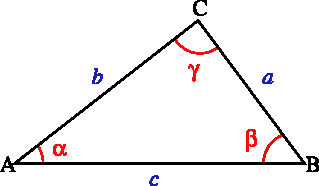
\includegraphics[scale=0.8]{./images/Triangle_with_notations_2.pdf}
\end{minipage}

\bigskip
(Here $\norm{a}$ denotes the norm: $\sqrt{\sum a_i^2} = \sqrt{\langle a,a\rangle }$). The dot product is $0$ if and only if the vectors are orthogonal to each other.

Now that we have defined vector spaces we want to study some linear transformations on them. Since vector spaces are closed under linear combination we'd like to have our transformation preserve that structure.

\begin{Def}[Linear Transformation] A linear transformation is (for our purposes) a mapping $T : \R^n \rightarrow \R^m$ with the following properties:

\begin{enumerate}
\item $T(\lambda w) = \lambda T(w)$
\item $T(v+w) = T(v)+T(w)$
\end{enumerate}
\end{Def}

Prominent examples for linear transformations are rotations and reflections around the origin. Note that if $T(\vec 0)\neq 0$ you automatically know that it's not a linear transformation.

If we use a standard basis for our vector space we can easily represent linear transformations by their effects on the basis. Just map every basis vector to its image and write the results in a matrix. 

\begin{Ex}[Reflection] Suppose we want to reflect every vector in $\R^2$ at the x-axis. If we use the standard base $V = \{(1,0),(0,1)\}$ and compute its reflection $V'=\{(1,0),(0,-1)\}$ we get the matrix

\[R = \begin{pmatrix}
1 & 0 \\
0 & -1
\end{pmatrix}\]

Multiplying a vector with that matrix we get its reflection. Just in case: Matrix multiplication

\[\begin{pmatrix}
a_{11} & a_{12} & \ldots & a_{1n}\\
a_{21} & a_{22} & \ldots & a_{2n}\\
\vdots \\
a_{m1} & a_{m2} & \ldots & a_{mn}
\end{pmatrix} * \begin{pmatrix}x_1\\x_2\\\vdots\\x_n\end{pmatrix} =\begin{pmatrix} \sum_{i=1}^n a_{1i}x_i\\ \sum_{i=1}^n a_{2i}x_i\\\vdots\\\sum_{i=1}^n a_{mi}x_i\end{pmatrix}\]

\end{Ex}

Note that for two transformations $f,g$ and their matrices $A,B$ we have
\[\forall \vec v:\ (f\circ g)(v) = (AB)v\]

\begin{Def}[Kernel of a matrix] 
 The kernel of a matrix $A$ is the set of all vectors $x$ with
$$Ax=0$$
\end{Def}

\begin{Def}[Rank of a matrix]
 The rank of a matrix $A$ is the number of linearly independent columns or rows of $A$. The column and row rank is always the same. In other words the row (column) rank is the dimension of the subspace spanned by the rows of $A$. A matrix $A^{m \times n}$ is said to have a full rank if $rank(A)=min(m,n)$
\end{Def}

If a matrix $A$ has full rank its kernel has dimension 0 and any system of equations $A x=b$ has a unique solution $A^{-1}b$. You can invert such matrices for example by using a Gauss-Jordan elimination. If the matrix is sparse it may be faster to calculate the inverse by

\[A^{-1} = \frac{1}{\det A} \tilde A \qquad \tilde a_{ij} = (-1)^{i+j} \det A_{ji}\]

Where $A_{ji}$ is the matrix $A$ without the $i$-th row and the $j$-th column and $\det A$ is the determinant of the matrix. It can be computed recursively:

\[\det A = \sum_{i=1}^n a_{ij} \cdot (-1)^{i+j} \det A_{ij} = \sum_{j=1}^n a_{ij} \cdot (-1)^{i+j} \det A_{ij} \]

For example
\[\det \begin{pmatrix} 
3 & 9 & 1\\
2 & 5 & 4\\
-2 & 8 & 7\end{pmatrix} \stackrel{i=2}{=}
-2\cdot \det \underbrace{\begin{pmatrix} 
9 & 1\\ 
8 & 7\end{pmatrix}}_{A_{21}} + 
5\cdot \det \underbrace{\begin{pmatrix}
3 & 1\\
-2 & 7\end{pmatrix}}_{A_{22}} -
4\cdot \det \underbrace{\begin{pmatrix} 
3 & 9\\ 
-2 & 8\end{pmatrix}}_{A_{23}}= -163\]

Here we fixed the second row and iterated over the columns. Since we multiply by $a_{ij}$ in each recursion step this procedure is fast if there are lots of zeros in the matrix.


\marginpar{Lecture 1}
\section{Introduction and Examples}

\marginpar{Lecture 2}
\section{Solving Linear Programs}
A linear program in general has the form:
\begin{eqnarray*}
\text{minimize:}& \vec c \cdot \vec x \\
\text{subject to:} & A \cdot \vec x \geq \vec b
\end{eqnarray*}
$x=\{x_1,x_2,..,x_n\}$ is an vector of variables in $\R$. $x$ together with the vector $c \in \R^n$ is the objective function.
$A^{m \times n}$ together with $x\in \R^m$ and $b \in \R^m$is the system of inequation which describes the constrains.
%From now on we'll characterize the system of inequation by a matrix and a vector. $A\vec x \geq \vec b$. The objective function can also be written in vector form $\min \vec c \vec x$, where $c$ is the cost vector.

Solving LPs with just two variables is rather easy. We can use a graphical approach in two dimensions. The constraints define halfplanes in the 2D space. The feasible region of the problem is then the intersection of all the halfplanes. The cost vector now defines a halfspace of its own (i.e. lines with equivalent costs) that can be shifted around by choosing different $x$. If $x$ lies within the feasible region we get a feasible solution. The goal is to shift the lines as far in negative $c$ direction as possible without leaving the feasible region. See figure \ref{Fig:graphSolutionEx}.

\begin{figure}[hbt]
\begin{minipage}[hbt]{0.4\linewidth}
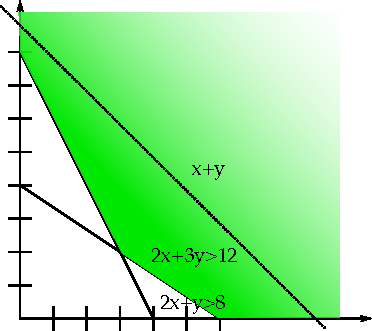
\includegraphics{./images/graphSolutionEx.pdf}
\end{minipage}
\hfill
\begin{minipage}[hbt]{0.4\linewidth}
\begin{align*}
\min x+y\\
2x+y\geq 8\\
2x+3y\geq 12
\end{align*}
\end{minipage}
\caption{An example for a graphical solution of an LP. The optimal solution is (3,2)}
\label{Fig:graphSolutionEx}
\end{figure}

How can we derive an algorithm from this method? We use the idea of sliding down, but just look at the corners of the feasible region, to get discrete steps (continuous sliding can't be implemented well). We start with any corner of the feasible region (a basic feasible solution) and look at its neighbors. Should they have a better objective value we move, else we're finished. 

To formalize the intuition from the 2D-space we need a notion of a corner in a (usually high dimensional) feasible region. To use it in a algorithm it should be a non-graphical definition. First we give some general definitions and then three different alternative definitions of a corner. We finish by proving that they are all equivalent.

\begin{Def}[Polyhedron] A set in $\R^n$ whose members obey a set of linear inequalities
\[\{x\in \R^n | Ax \geq b\} \qquad A\in \R^{m\times n},\ b\in \R^m\]
\end{Def}

\begin{Def}[Hyperplane, Hyperspace] \label{Def:hyperPlaneSpace} Let $a,x\in \R^n$, $a\neq 0$. 
\begin{enumerate}
\item $\{x|ax=b\}$ is a \emph{hyperplane} (a line in 2D)
\item $\{x|ax\geq b\}$ is a \emph{halfspace} (halfplane in 2D)
\end{enumerate}
\end{Def}

With definition \ref{Def:hyperPlaneSpace} we can say that a polyhedron is an intersection of a bunch of halfspaces.

\begin{Def}[Convex Sets] A subset $S \subseteq \R^n$ is called \emph{convex} if any convex combination between two points (graphically: points on a line between those points) is contained in the set. See figure \ref{Fig:convexNotConvex}
\[\forall \lambda \in [0,1], \forall x,y\in S: \lambda x + (1-\lambda) y \in S\]
\end{Def}

\begin{figure}[hbt]
\begin{center}
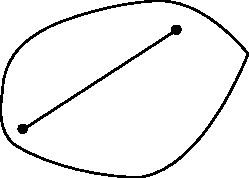
\includegraphics{./images/convex.pdf}\hspace{2cm}
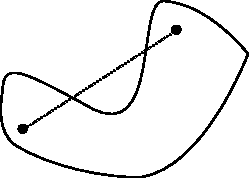
\includegraphics{./images/notConvex.pdf}
\end{center}
\caption{Graphical example for a convex and a non convex set (with non linear borders)}
\label{Fig:convexNotConvex}
\end{figure}

Convex sets have a lot of nice properties. Luckily feasible regions are always convex. This is the main reason why we can efficiently solve LPs. 

\subsection*{Corners}
The following three definitions formalize the notion of a corner.

\begin{Def}[Vertex]\label{Def:Vertex} Let P be a polyhedron. A vector $x\in P$ is a \emph{vertex} of P if $\exists \vec c\in \R^n$
 s.t. $cx < cy$ for all $y\in P, y \neq x $; that is $x$ is the minimal point for some cost vector (the unique optimal solution for some LP with the feasible set P). See figure \ref{Fig:vertex}
\end{Def}

\begin{figure}[hbt]
\begin{center}
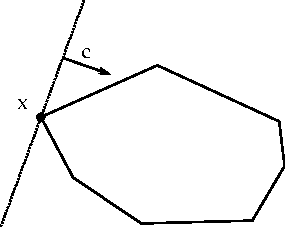
\includegraphics{./images/vertex.pdf}
\end{center}
\caption{A vertex $x$ is the optimal solution for a cost vector $c$}
\label{Fig:vertex}
\end{figure}

\begin{Def}[Extreme Point]\label{Def:ExtremePoint} An \emph{extreme point} of a polyhedron P is a vector $x\in P$ s.t. $x$ is not a convex combination of any two vectors $y,z\in P$ different from $x$. 
\end{Def}
Example: In 2D we can always select the two adjacent corners of a point $x$ on the edge of $P$ iff $x$ is not a corner. Then $x$ will be on the line between the two corners. 

\begin{Def}[Active Constraint]\label{Def:ActiveConstraint} Let $P$ be a polyhedron that is defined by some linear inequalities $a_i$: $P=\{x|a_ix\geq b_i\}$. We'll say that the $i$-th constraint is \emph{active} at a point $x$ if we have equality there $a_ix = b_i$
\end{Def}

\begin{Def}[Basic Feasible Solution]\label{Def:BFS} Let $P$ be a polyhedron in $n$ dimensions. Then $x\in P$ is a \emph{basic feasible solution} if the set of active constraints has full rank, that is there are $n$ linearly independent active constraint vectors at the point $x$. See figure \ref{Fig:bfsActiveConstraints}
\[\mbox{rank}(\{a_i\in \R^n|a_ix=b_i\}) = n\]

In particular there never is a b.f.s. if we have less than $n$ constraints. (Example: A line in 2D-Space or a plane in 3D-Space)
\end{Def}

\begin{figure}[hbt]
\begin{center}
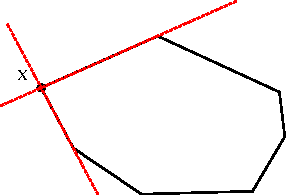
\includegraphics{./images/bfs.pdf}
\end{center}
\caption{Two constraints (red lines) are active at $x$. It's a basic feasible solution}
\label{Fig:bfsActiveConstraints}
\end{figure}

Now we want to prove that the three definitions \ref{Def:Vertex}, \ref{Def:ExtremePoint} and \ref{Def:BFS} are all equivalent to each other.

\begin{thm} \label{Thm:cornerEquiv} Let $P$ be a polyhedron and $x\in P$. The following are equivalent
\begin{enumerate}
\item $x$ is a vertex
\item $x$ is an extreme point
\item $x$ is a basic feasible solution
\end{enumerate}
\end{thm}

\begin{pr}[Theorem \ref{Thm:cornerEquiv}] The proof goes in three steps
\begin{itemize}
\item vertex $\Rightarrow$ extreme point: Proof by contraposition. Assume the existence of $y,z \in P$ s.t. $y,z\neq x$ with $x= \lambda y + (1-\lambda )z$. That is, $x$ is not an extreme point (definition \ref{Def:ExtremePoint}). We want to show that it's not a vertex either.

From definition a vertex (def. \ref{Def:Vertex}) we know that some $c$ should exist such that $c x < c \lambda y  + c (1-\lambda) z$. That however is a contradiction to the assumption $x= \lambda y + (1-\lambda )z$.
\begin{align*}
cx &= \lambda cy +(1-\lambda)cz\\
   &< \lambda cx + (1-\lambda)cx\\
   &< cx
\end{align*}

\item extreme point $\Rightarrow$ bsf (proof by contraposition; we show $\neg \text{bsf} \Rightarrow \neg \text{extreme point}$): Suppose $x\in P$ is not a basic feasible solution. Let $B$ be a matrix of active constraints at $x$ and $C$ the matrix of the inactive constraints such that $Bx=d$, $Cx\gneq f$ and $A = \left[B\atop C\right]$. Since $x$ is not a bfs the matrix $B$ hasn't full rank and its kernel is nonempty. Hence

\[\exists \delta \in \R^n, \delta \neq 0:\ B\delta =0\]

See figure \ref{Fig:extremeBfs}. With $\delta$ we define two vectors:

\[y=x+\epsilon \delta \quad z = x-\epsilon \delta\]

Note that $x=(z+y)/2$. That means that $x$ is not an extreme point if $z,y \in P$, because $x$ is a convex combination of the two. Consider 

\[Bz = B(x+\epsilon \delta) = Bx + \epsilon B\delta = Bx\]

Since $B\delta = 0$ the active constraints are still active. For the inactive constraints we have some slack before we leave the polyhedron (We can move around on the red line in figure \ref{Fig:extremeBfs}). If we choose $\epsilon$ small enough we're still within. It suffices to choose $\epsilon$ such that 

\[\forall i: \epsilon |c_i z| < c_i x - f_i\qquad \vec c_i\in C,\ f_i \in \vec f\]

Hence $z$ (and analogous $y$) are still in the polyhedron and $x$ is not an extreme point.

\begin{figure}
\begin{center}
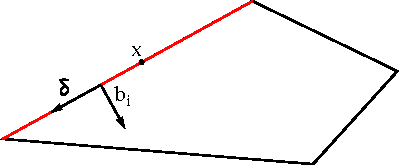
\includegraphics{./images/extreme_bfs.pdf}
\end{center}
\caption{$x$, active constraint $b_i$ and orthogonal vector $\delta$}
\label{Fig:extremeBfs}
\end{figure}

\item bfs $\Rightarrow$ vertex: Suppose $x$ is a bsf. Let $I$ be the indices of all active constraints and $c=\sum_{i \in I} a_i$. Then $c x = \sum_{i \in I} b_i$, since for each $a_i x \geq b_i $ the inequality is tight (see def. \ref{Def:ActiveConstraint}). 

Also $\forall y\in P, i\in I$ we have $a_i y \geq b_i$. Therefore $c y \geq c x$. The greater then is sharp as $x$ is the unique solution to the active constraints because it's a bfs and the system of active constraints has full rank, i.e. if n-lines cross in n-dimensional space they do so at \emph{one} point. (Theorem 2.2 in the Linear Optimization book). So $x$ is the optimal solution for some LP and hence a vertex.
\end{itemize}

\subsection*{Standard Form}
A LP in standard form\footnote{Cormen et al. name this slack-form (Schlupfform)} is of the form:
\begin{eqnarray*}
\text{minimize:}& \vec c \cdot \vec x \\
\text{subject to:} & A \cdot \vec x = \vec b \\
& x\geq0
\end{eqnarray*}

Any LP can be transformed into an equivalent LP in standard form. Two steps are needed for this, one to add non negativity constraints for all variables and a second to transform any inequalities into a equalities.

\paragraph*{Add non negativity constraints:} Suppose a variable $x$ has no non-negativity constraint. $x$ can be replaced with two variables $x'$ and $x''$ such that $x=x'-x''$ and $x',x''\geq 0$, as any negative number can be written as a combination of two non negative numbers.

\paragraph*{Remove inequalities:} Suppose a constraint $a$ to be $x_1+2x_2 \geq 15$. By adding a new variable $s\in \R$ and the constraint $a-s=15$ we can remove the inequality. So by adding a new vector $s\in \R^n$ with $A \cdot \vec x - s = \vec b$ the inequalities can be removed.

\end{pr}

\marginpar{Lecture 3}
To get a better intuition for the different definitions of a corner, we'll use them for some things that are not directly related to solving LPs.

\subsection*{Convex Hulls}

\begin{Def}(Convex Hull) Let $x_1,\ldots,x_k$ be some vectors in $\R^n$. The convex hull of these vectors is
\[\mbox{CH}(\{x_1,\ldots,x_k\}) = \left\{\sum _{i=1}^k \lambda_i x_i \left| \sum_{i=1}^k \lambda_i =1,\ \lambda_i\geq 0\right.\right\}\]
\end{Def}

Here we generalise the notion of convex combination to use more than two points. Intuitively if we have a bunch of points in 2D we get all the points that lie within the polygon that is spanned by the points on the CH, see figure \ref{Fig:convexHull}.

\begin{figure}[hbt]
\begin{center}
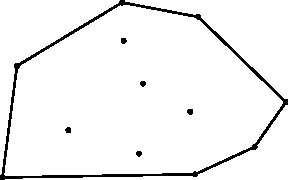
\includegraphics{./images/convex_hull.pdf}
\end{center}
\caption{The convex hull of a set of points}
\label{Fig:convexHull}
\end{figure}

This definition allows us to come up with a different definition of a polyhedron. In contrast to definition \ref{Def:polyhedron} the convex hull definition allows us to have a more geometric view of the problem.

\begin{Def}[Bounded Polyhedra] A bounded polyhedron lies within a finite bounding box, see figure \ref{Fig:bounded_unbounded}. More formally

\[\forall x\in P,d\in \R^n, \forall \lambda > 0: x+\lambda d \not \in P\]

For any line from a point inside the polyhedron we eventually leave the polyhedron
\end{Def}

\begin{figure}[hbt]
\begin{center}
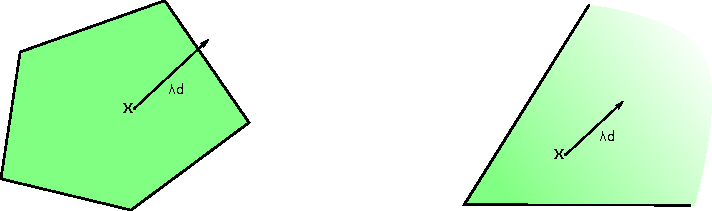
\includegraphics{./images/bounded_unbounded.pdf}
\end{center}
\caption{A bounded (left) and an unbounded (right) polyhedron}
\label{Fig:bounded_unbounded}
\end{figure}

\begin{thm}\label{Thm:CH_polyhedron} Let $P$ be a non-empty bounded polyhedron. Then $P=$\mbox{CH}(extreme points $P$)
\end{thm}

\begin{pr}[Theorem \ref{Thm:CH_polyhedron}] We prove equality by showing mutual inclusion:
\begin{description}
%#todo
%sieht unschoen aus, muessten wir anders formatieren
\item[$\text{CH(extreme points of P)} \subseteq \text{P}$] As polyhedra are convex sets. Every convex combination of extreme points must be in $P$.\\ 
\item[$\text{P} \subseteq \text{CH(extreme points of P)}$]:  From the definition we know that all convex combinations of two points are still in P. We generalise to the new kind of convex combination that includes several vectors. 

Let $x\in P$. Since $P$ is a polyhedron $x$ is a solution of the system of inequations $Ax\geq b$ (def. \ref{Def:polyhedron}). As in the proof for theorem \ref{Thm:cornerEquiv} we separate $A$ into the matrix $B$ of active constraint and $D$ of inactive constraints, with $Bx=d$, $Dx>f$. If the rank of $B$ is $n$, $x$ is an extreme point by definition and we're done. 

The other possibility is $\rank B=k$ and $k<n$. We use the same trick as in proof \ref{Thm:cornerEquiv} to find two new points. Since the matrix hasn't full rank, there has to be $\delta \neq 0$ such that $B\delta = 0$. As before we build two vectors $x_1 = x+ \epsilon_1 \delta$, $x_2=x-\epsilon_2 \delta$. 

Now we want to get from these points somehow to extreme points, as we want to prove that we can use extreme points to represent every point in $P$. We choose $\epsilon>0$ as the largest value such that $x_1$ is still a feasible solution, that is, we follow a line through $x$ until we reach a boundary of the polyhedron. See figure \ref{Fig:convCombExPoints} for a graphical representation of the process in a 2D-Polyhedron.

\begin{figure}[hbt]
\begin{center}
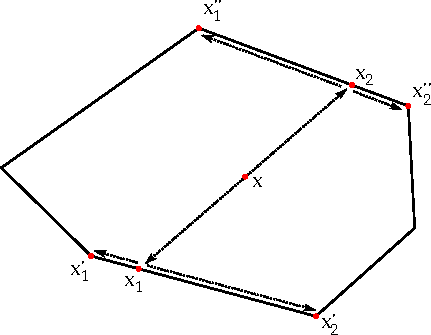
\includegraphics{./images/convex_comb_extr_points.pdf}
\end{center}
\caption{$x$ can be written as a convex combination of $x_1',x_2', x_1''$ and $x_2''$}
\label{Fig:convCombExPoints}
\end{figure}

Such an $\epsilon$ has to exist, since the polyhedron is bounded and therefore every line eventually crosses a boundary.\footnote{The calculation we did in the lecture to find $\epsilon_{1,2}$ seems dubious to the authors. We'll investigate.} Choosing $\epsilon$ like this implies that some constraint $a_i$ in $D$ has to become active for $x_1$ and the same holds with a different $a_i$ for $x_2$. Moving in direction $\delta$ doesn't affect the constraints that already were active, since $\delta$ is in the kernel of $B$. So we increase the number of active constraints and can extend $B$ to 

\[\begin{pmatrix}B\\ a_i\end{pmatrix}\] 

The rank of the new $B$ has to be $k+1$ since $\delta$ was orthogonal to all the vectors in $B$, as $B\delta=0$ (and hence all vectors in $\text{span } B$), but it is not orthogonal to $a_i$, or we wouldn't have hit that constraint by moving in direction $\delta$.

We have now reduced the problem of finding extreme points to represent $x \in P$ to the problem of finding some for $x_1,x_2 \in P$. However we increased the number of active constraints for $x_1,x_2$ (in 2D: we moved them on an edge). This process can be repeated for $x_1$ and $x_2$ until the respective $B$ has full rank and we arrived at some extreme points. For figure \ref{Thm:CH_polyhedron} the process is repeated three times, for $x,x_1$ and $x_2$. 
Since all the points from the beginning can be recursively written by a convex combination of the new points and we end up at an extreme point, the original $x$ can transitively be written by a convex combination of extreme points.
\end{description}

% Ich hab noch drüber nachgedacht und die Rechnung da in der Tat komisch zu sein. Er (oder ich :D) scheint sich zwischendurch verrechnet zu haben. Wir haben nicht genug info das zu lösen:
%
% x&=\lambda x_1+(1-\lambda)x_2 % ist die Linie zwischen x1,2 auf der x liegt. Wir wollen x_1,2 soweit nach außen schieben dass wir am Rand ankommen
% x&=\lambda (x+\epsilon_1\delta) + (1-\lambda)(x-\epsilon_2\delta) % ist das selbe nochmal neu geschrieben. Jetzt wollen wir nach den epsilons auflösen ???
% x-\lambda x - (1-\lambda) x = \lambda \epsilon_1\delta + (1-\lambda)\epsilon_2\delta
% x -\lambda x - x +\lambda x  = \epsilon_1\delta +\epsilon_2\delta
% 0 = \epsilon_1 \delta + \epsilon_2\delta
% ???
% Profit.



%In particular choose \label{wieso}
%\begin{align*}
%x&=\lambda x_1+(1-\lambda)x_2\\
%&=x+\underbrace{\lambda \epsilon_1\delta -(1-\lambda)\epsilon_2\delta}_{\stackrel{!}{=}0}\\
%&\Rightarrow \lambda = \frac{\epsilon_2}{\epsilon_1+\epsilon_2}
%\end{align*}

\end{pr}

\begin{cor}\label{Cor:always_extreme_points} Let $P$ be a non-empty bounded polyhedron. Then the LP $\min cx$ s.t. $x\in P$ always has an optimal solution that is an extreme point of $P$.
\end{cor}

Intuitively this is true, as given an optimal solution, which is not an extreme point, we could always go into the direction of a constraint which is not tight. Such a constraint must exist, as otherwise we would be at an extreme point. 

\begin{pr}[Corollary \ref{Cor:always_extreme_points}] %(from the book 'Linear Optimization') 
Start with some optimal solution $x^*$. Write it as a convex combination of extreme points 
\[x^* = \sum_{i=1}^x \lambda_i y_i \qquad \text{s.t. } y_i \text{ is an extreme point}\]
We want to prove that there is an extreme point $y_i$ such that the cost $v$ are the same as in $x^{*}$, that is:

\[v = cx^* = cy_i\]

Obviously $cy_i\geq v$ since $x^*$ is an optimal solution. It can't be strictly greater for all $y_i$ or 
\[c\sum_{i=1}^x \lambda_i y_i \gneq v\]
since the $\lambda_i$ are greater than zero and $\sum_i \lambda_i =1$. This would be a contradiction since $x^*=\sum_{i=1}^x \lambda_i y_i$. So there has to be at least one extreme point $y_i$ for which $cy_i=v$.
\end{pr}

Corollary \ref{Cor:always_extreme_points} gives us the nice result that we can transform the problem of optimising an LP to a discrete problem with finitely (albeit exponentially) many candidate solutions. This will of course be very useful in designing an algorithm for solving them.

\subsection*{Fourier-Motzkin elimination}

In this section we're interested in computing representations of projections of polyhedra. See figure \ref{Fig:polyhedron_proj} for an example.

\begin{figure}[hbt]
\begin{center}
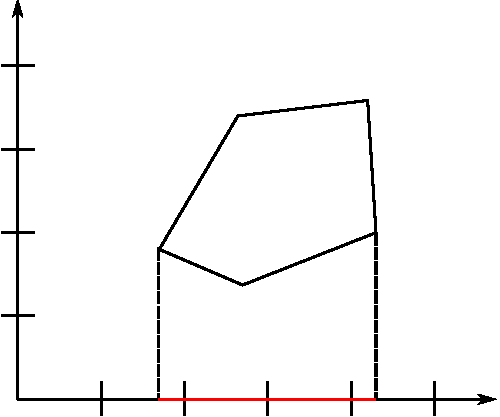
\includegraphics[width=0.3\textwidth]{./images/polyhedron_proj.pdf}
\end{center}
\caption{A projection which removes one of the two dimensions.}
\label{Fig:polyhedron_proj}
\end{figure}

\begin{Def} The projection $x=(\nthings{x})$ onto its first $k$ coordinates is $\pi_k(x) = (x_1,\ldots, x_k)$. 

Let $S\subseteq \R^n$ then the projection on the first $k$ components is

\[\pi_k(S)=\{\pi_k{x}|x\in S\}\]
\end{Def}

Of course that definition is not particularly useful in actually constructing the projection. The Fourier-Motzkin elimination computes the projection for polyhedra. We start with our usual characterisation of a polyhedron $P=\{x|Ax\geq b_i\}$ and want to find a different matrix $A'$ s.t. we get $\pi_{n-1}(P)$. Generalizing to $\pi_k$ is then of course easy.

\subsubsection*{Example of Fourier-Motzkin elimination}
Figure \ref{Fig:motzkinExample} shows an example of the Fourier-Motzkin elimination. The LP used for the example is:
\begin{eqnarray*}
c_1 & -0,5x + y & \leq 3 \\
c_2 & 2x + y & \leq 6 \\
c_3 & x+3y & \geq 6 \\
c_4 & x+y & \geq 2
\end{eqnarray*}
Those constraints can be rewritten to:
\begin{eqnarray*}
c_1 & \frac{1}{2}x + 3  & \geq y \\
c_2 & -2x+6 & \geq y \\
c_3 & y & \geq -\frac{1}{3}x+2 \\
c_4 & y & \geq -x+2
\end{eqnarray*}
Writting them this way has the advantage of ordering them around $y$. With this information we can build a new LP, which constraints are only on the x-dimension. The constraints are all the ordered pairs of around $y$.
\begin{eqnarray*}
c_1 \geq c_3: & \frac{1}{2}x + 3 & \geq -\frac{1}{3}x+2  \\
c_2 \geq c_3: & -2x+6 &  \geq -\frac{1}{3}x+2 \\
c_1 \geq c_4: & \frac{1}{2}x + 3   & \geq -\frac{1}{3}x+2 \\
c_2 \geq c_4: & -2x+6 & \geq -x+2
\end{eqnarray*}
Those constrains are shown in figure \ref{Fig:motzkinExample} below the x-axis with dashed lines. Note that we're only interested in the red part. So the two constraint $c_2 \geq c_3$ and $c_1 \geq c_4$ would be enough. As there is no efficent way to find those two constraints we have to keep all of them. 

\begin{figure}[hbt]
\begin{center}
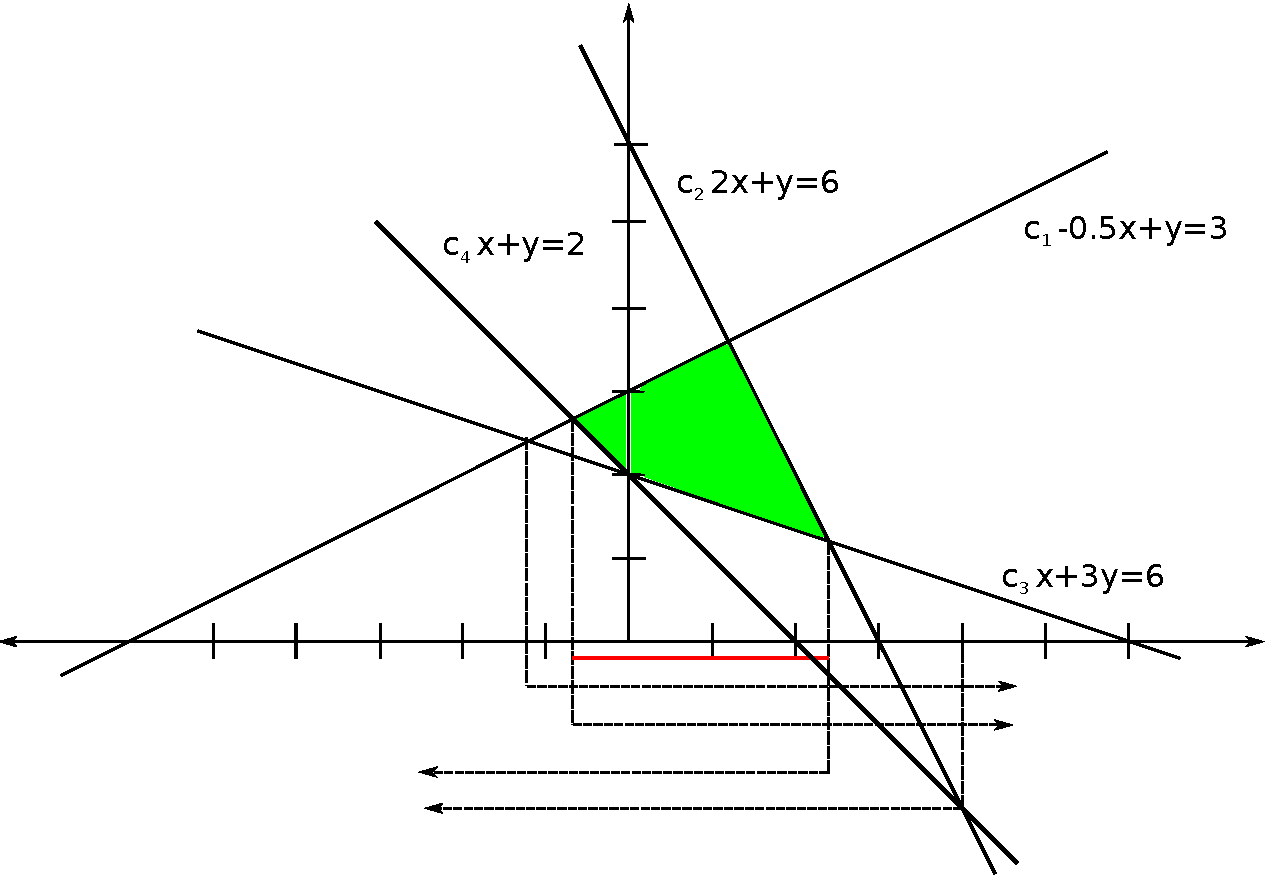
\includegraphics[width=0.8\textwidth]{./images/motzkin.pdf} %TODO die gestrichelten Linien mit c_1,..,4 beschriften 
\end{center}
\caption{A projection, which removes one of the two dimensions. The result is shown in red.}
\label{Fig:motzkinExample}
\end{figure}

\subsubsection*{General case}
We want to classify the constraints $a_i$ into three kinds. Let $\overline a = \pi_{n-1}(a)$ then we can write  

\[P=\left\{x\left| \begin{array}{cr}
\overline a_i\overline x +a_{in}x_n \geq b_i & i\in T_1\\
\overline a_i\overline x +a_{in}x_n \geq b_i & i\in T_2\\
\overline a_i\overline x \geq b_i & i\in T_3\\
\end{array}\right.\right\}\]

With 
$$\forall i\in T_1: a_{in}>0$$ $$\forall i\in T_2: a_{in}<0$$ $$ \forall i\in T_3: a_{in}=0 $$

From that form we rewrite the polyhedron by dividing with $\overline a_{in}$ if $\overline a_{in}\neq 0$. The $f_i$ are vectors and the $d_i$ are scalars. 

\begin{equation}\label{For:Motz1}x_n \geq  d_i + f_i \bar x : i \in T_1 \end{equation}
\begin{equation}\label{For:Motz2}x_n \leq  d_i+f_i \bar x : i \in T_2 \end{equation}
\begin{equation}\label{For:Motz3}0 \geq  d_i+f_i \bar x : i \in T_3 \end{equation}

%\[P \{i\in T_1 \wedge x_n \geq d_i + f_i \bar x \vee i\in T_2 \wedge x_n \leq d_i + f_i \bar x \vee i\in T_3 \wedge 0 \leq d_i + f_i \bar x\}\]

Then we can write the projection $\overline P=Q$ as\footnote{Adrians lecture notes as well as mine read: $\{d_i+f_i\bar x \leq d_j+f_j\bar x\ \forall i\in T_2, j\in T_1 $. The book says $\geq$ and $T_2\geq x_n \geq T_1$}

\begin{eqnarray*}
\{d_i+f_i\bar x & \geq d_j+f_j\bar x\ & \forall i\in T_2, j\in T_1  \\
d_i+f_i\bar x & \geq 0\ & \forall i\in T_3\}
\end{eqnarray*}

%$$\{d_i+f_i\bar x \geq d_j+f_j\bar x\ \forall i\in T_2, j\in T_1 $$ 
%$$d_i+f_i\bar x \geq 0\ \forall i\in T_3\}$$

Herein lies the problem of the algorithm. We introduce a new constraint for every pair of constraints from $T_1,T_2$. Hence in every iteration the number of constraints $c$ can grow on the order of $(\frac{c}{2})^2$.

\subsubsection*{Proof of correctness}
\begin{pr} To prove the correctness of the Fourier-Motzkin elimination we need to show that the result $Q$ of the algorithm is equal to $\pi_{n-1}(P)$. We do this by showing $\pi_{n-1}(P) \subset Q$ and $Q \subset \pi_{n-1}(P)$.
\begin{enumerate}

\item $\bar x \in \pi_{n-1}(P) \Rightarrow \bar x\in Q$. That means 
\[\exists x_n: \left[{\bar x}\atop{x_n}\right] \in P \Rightarrow {{\max_{i\in T_1} d_i +f_i \bar x \leq x_n} \atop {\min_{i\in T_2} d_i+fi\bar x \geq x_n}}\]
Therefore the constraints \ref{For:Motz1}, \ref{For:Motz2} and \ref{For:Motz3} are satisfied. It follows that $\bar x \in Q$. 

\item $\bar x \in Q \Rightarrow \bar x \in \pi_{n-1}(P)$. Choosing $x_n$ as 
\[x_n \in [\max_{i\in T_1} d_i+f_i \bar x, \min_{i\in T_2} d_i+f_i \bar x]\]
does the trick, as $(\bar x, x)$ then satisfies constrains \ref{For:Motz1}, \ref{For:Motz2} and \ref{For:Motz3} and therefore is in $P$.

\end{enumerate}
\end{pr}

There are a lot of interesting applications for these projections:

\begin{thm}\label{Thm:linTransPoly} Let $P\in \R^n$ be a polyhedron and $A\in \R^{m\times n}$ be a matrix. Then the set
\[Q=\{Ax|x\in P\}\]
is also a polyhedron.
\end{thm}

In 2D this is intuitively clear: applying linear transformations on polygons results in distorted, rotated etc. polygons. For higher dimensions it follows from the projections:

\begin{pr}[Theorem \ref{Thm:linTransPoly}] For $P$ we have

\[Q=\{(Ax,x)\in \R^{m+n}| x\in P, P\text{ is a polyhedron in } \R^{n}, A \in \R^{m \times n}\}\]  %this is actually not that intuitive for me. Why is this a polyhedron?

is a polyhedron. Then $\pi_m(Q)$ is also a polyhedron.
\end{pr}

\begin{cor} Let $x_1,x_2,\ldots, x_k \in \R^n$, then CH($x_1,x_2,\ldots, x_k$) is a polyhedron\end{cor}

\paragraph*{Optimal value} We can use the projections to find the optimal value for an LP (not the optimal solution though). Suppose we're given a LP in the usual form, $\min cx$ s.t. $Ax\geq b$. We construct the following polyhedron P:

\begin{eqnarray*}
 & (x_0,\ldots,x_n) & \\
s.t. & A(x_0,\ldots,x_n)^{\mbox{T}} & \geq b \\
& c(x_0,\ldots,x_n)^{\mbox{T}} & = x_0
\end{eqnarray*}

Define $Q = \pi_1(P)$. We can find $Q$ with the Fourier-Motzkin elimination. If $Q$ is not feasible, $P$ is empty. Else we can choose the biggest $b_i$ such that $x_0\geq b_i$ or the smallest $b_i$ such that $x_0 \leq b_i$, depending on the type of constraints we have. That is the optimal value.

\begin{thm}[Farkas' lemma] Let $A\in \R^{m\times n}$ and $b\in \R^m$. Then either 
\begin{itemize}
\item $\exists x\in \R^n: Ax\geq b$ or
\item $\exists y\in \R^m, y\geq 0, y^{\mbox{T}}A=0: y\cdot b>0$
\end{itemize}
\end{thm} 

This theorem is very nice if we want to check if some system of inequalities is feasible. We just have to find the vector $y$. This lemma can be proven by our earlier results. (Sketch:) We start with the polygon $P$ and use a projection to get rid of the last dimension of $P$. By that we get another matrix $B$ and another vector $d$. We get the new inequalities by combining those from the original polyhedron. Instead of actually doing the projection to a lower dimension we can replace the last element by 0. You can show that $[B0]=DA$ (no proof). You can repeat that process until you get a matrix $F$ such that $FA=0$. The system is infeasible if you end up with a negative rhs for a constraint, since all lhs will be 0.

\marginpar{Lecture 4}
\subsection{The simplex algorithm}
Recall that an LP is in standard form if

\begin{align*}
\min cx\\
Ax = b\\
x\geq 0
\end{align*}

and $A\in \R^{m\times n}$ has $m$ linearly independet rows. A basis $B\subseteq [1,n]$ is as set of $m$ indices such that $A_B$ has full rank $m$. It induces a basic solution

\[\begin{cases} x_B = A^{-1}_Bb\\ x_{\bar B} = 0\end{cases}\]

We say it is feasible if $x_B\geq 0$. Note that the $x_{\bar B}=0$ part makes $n-m$ non-negativity constraints active so that we actually are at a corner with $n$ active constraints in $n$ dimensions.

The simplex algorithm works by moving from corner to corner, always in the direction of better costs. At first we'll have some simplifying assumptions, to avoid the messy details:

\begin{enumerate}
\item The LP is in standard form (for conversion see \ref{Sec:standardForm})
\item Every feasible basis $A$ is non-degenerate. A basis $B$ is non-degenerate if $\forall b:\ x_B=A^{-1}_Bb \gneq 0$. Note the difference to $x_B\geq 0$ for general basic solutions. So it is forbidden that more than $n$ (those in $B$ and $>n-m$ non-negativity) constraints are active (in $n$ dimensions they can't all be linearly independet of course). 
\item We are given an initial feasible basis
\item The feasible region of the LP is bounded
\end{enumerate}

In the next lectures we'll remove those assumptions one after the other.

The algorithm works as follows:
\begin{lstlisting}
SIMPLEX-TAKE-I(A,b,c)

B <- find some feasible basis
// B=$\{b_1,b_2,\ldots, b_m\} \subseteq [1,\ldots, n]$
repeat 
    for $j\in [1,n]\backslash B$ and  $b_i \in B$
        D = B $\cup$ j $\backslash$ $b_i$
        if D is a basis then
            $x_B$ = $A^{-1}_B$b
            $y_D$ = $A_D^{-1}b$ // a bfs
            if ($y_D$ $\geq$ 0 and $c_Dy_D < c_Bx_B$)
                B = D
until B hasn't changed                
\end{lstlisting}

$D$ is build by removing one constraint from $B$ and adding another one that wasn't in there before. We then check if $D$ is non-singular. If so it induces a basic solution, we just have to check if it's feasible. If yes we check if the cost improves and move to $D$ if it does.

It will later turn out that we don't actually have to check every combination for $j$ and $b_i$. The choice of $b_i$ is uniquely determined.

We can't get the same basic solution from two different bases, if we have a non-degenerate LP. In the degenerate case this may very well happen:

\begin{align*}
x_2 + x_3 &= 1\\
x_1 - x_2 +x_4 &=0\\
x_1 + x_2 +x_5 &= 2\\
\end{align*}

% figure

The above system gives us the solution $(1,1,0,0,0)$ for three bases $\{1,2,3\},\{1,2,4\},\{1,2,5\}$. This happens because we have a point where three constraints are active, although we're in 2D. See figure \ref{Fig:degenerateLP}. It is easy to see that if we have two bases build from indices $k\in [1,\ldots,n]$ that give us the same solution one of the $x_k$ (a basic variable) has to be zero. %easy to see :S

%figure

We move from solution $x$ to solution $y$ along some vector $d$ ($y=x+\Theta d$). Have a look at figure \ref{Fig:movingToSolutions}. We do some observations on the vector $d$. 

\begin{itemize}
\item $d_k=0$ if $k\not \in B \cup j$, because we assumed all variables not in the basis (i.e. the non-basic variables) to be zero to make the non-negativity constraints active 
\item $d_j>0$ $(x_k=0, y_k=0)$. By choosing $\Theta$ accordingly we can scale this to be $d_j=1$
\item $Ad = 0$ ($Ad = (Ay-Ax)/\Theta = (b-b)/\Theta = 0)$
\end{itemize}

By using these observations we can directly calculate the $b_i$ we need to remove.

We can rewrite $A_d$ like follows and can use that to find the components of $d$:

\[A_d = A_B d_B+A_j = 0 \Rightarrow d_B = -A^{-1}_B A_j\]

We also want $y\geq 0$ so that we need

\[x_B - d_B = x_B - \Theta A_B^{-1} A_j \geq 0\]

Thet means if $d_{b_i}>0$ we are ok, however if $d_{b_i} <0$ then $x_{b_i} +\Theta_{b_i} \stackrel{!}{\geq} 0$ so $\Theta \leq \frac{-x_{b_i}}{d_{b_i}}$. We can do that by choosing

\[\Theta = \min_{{b_i\in B}\atop {d_{b_i} <0}} \left| \frac{x_{b_i}}{d_{b_i}}\right |\]

So the indices attaining the minimum will be the ones we'll have to take out. Because we assumed that the system is non degenerate there will be only one element actually attaining it. %why does non-degenerate imply that?

How does the cost change?

\[cy -cx = \Theta cd = \Theta(c_j+c_Bd_B) = \Theta(c_j - c_B^TA^{-1}_B A_j)\]

If $y$ was a solution that we move to we did that because $cy$ was smaller that $cx$. So $c_j - c_B^TA^{-1}_B A_j$ should be negative if we want to move to $y$

\begin{lstlisting}
SIMPLEX-TAKE-II (A,b,c)

B = some feasible basis
repeat 
    for $j\in \{1,\ldots,n\}\backslash B$ // $b_i$ is determined
        $d_B$ = $A^{-1}_B A_j$
        if $c_j - c_B^TA^{-1}_B A_j < 0$
            $b_i$ = index  s.t. $d_{b_i} <0$, 
                    minimizing $\left| \frac{x_{b_i}}{d_{b_i}}\right|$
            B = B $\cup$ j $\backslash$ $b_i$
until B hasn't changed
\end{lstlisting}

%todo rechnungen zwischen II und III

\begin{lstlisting}
SIMPLEX-TAKE-III (A,b,c)

B = some feasible solution
repeat
    $\bar c$ = c - $c^T_B A^{-1}_BA$ //reduced cost vector
    if $\exists j:{\bar c}_j<0$ 
        u = $A^{-1}_B A_j$ // dimension m
        $b_i$ = index in B s.t. $u_i >0$ 
                minimizes  $x_{b_i}/u_i$
        B = B $\cup$ j $\backslash b_i$ 
until B hasn't changed 
// $\bar c \geq 0$ 
\end{lstlisting}

The algorithm always terminates because the assumptions ensure that we always have a optimal solution and we improve our solution in every step.

\begin{thm}\label{Pr:simplexIIIopt} Let B be a basis. If $x_B=A^{-1}_Bb\geq 0$ and $\bar c=c-c_B^{T}A_B^{-1}A_j$ then $B$ is optimal.\end{thm}

\begin{pr}[Theorem \ref{Pr:simplexIIIopt}] Let $x$ be the bsf induced by $B$, $y$ be some feasible solution. We want to argue that the cost of $x$ is smaller than the cost of $y$. Let $d=y-x$ then 
\[cd = c_Bd_B + \sum_{j\in \bar B} c_jd_j \] 

To be continued
\end{pr}

\marginpar{Lecture 5}
\subsection*{Tableau Implementation}

\textcolor{red}{Make sure to understand this part, it will be in the midterm.}

Imagine we had the following table at the beginning of an iteration:

\begin{center}
%c is a row vector!
\begin{tabular}{c|c}
$-c_BA_B^{-1}b$ & $c-c_BA_B^{-1}A$\\\hline %don't transpose, it's a rowvector
$A^{-1}_B b$ & $A_B^{-1}A$
\end{tabular}
\end{center}

In the lower right cell we can get the vector $u$. By dividing the components of $u$ by the number in the column we selected to be introduced into the basis we can find the basic index we need to kick out. It will turn out that computing the new inverse matrices it easy, as they change only in one column from iteration to iteration.

Suppose we have $A_B^{-1}$ and want to find $A_D^{-1}$, where $D=B\cup j \backslash b_i$. Suppose we already had the correct solution with $A_B^{-1}$ 

\[A_B^{-1}A_D = \left[ A_B^{-1}A_{b_i}\ldots A_B^{-1}A_j\ldots A_B^{-1}A_m\right] = \left[ e_1,e_2, \ldots, e_{i-1}, \underbrace{A_B^{-1}A_j}_{=u}, e_{i+1},\ldots, e_m\right]\]

So it's not the correct inverse, but the difference is very small. So we want to find a correction matrix $R$ that gives us the right answer. It is the identity matrix, except for the column that is wrong.

\[R= \begin{pmatrix} 
1 & \ldots & -u_1/u_i & \ldots \\
0 & \ldots & -u_2/u_i & \ldots \\
\vdots & \ddots & \vdots \\
& & 1/u_i & \ldots\\
\vdots & &\vdots &\ddots\\
& & & \ldots & 1
\end{pmatrix}\]

Then we get $RA_B^{-1} = A_D^{-1}$. You can find $R$ yourself by doing gaussian elimination on $A_B^{-1}A_D$ and accumulating the transformation matrices.

\begin{Ex} So now forget for a moment that fancy matrix stuff and see what's going on when you solve an LP by hand.

Suppose we have the following LP

\begin{align*}
\min \qquad& -10 x_1 - 12 x_2 - 12 x_3\\
\text{s.t.}\qquad & x_1 + 2 x_2 +2 x_3 \leq 20\\
& 2x_1 + x_2 + 2 x_3\leq 20\\
& 2x_1 + 2 x_2 + x_3\leq 20\\
& x_1,x_2,x_3 \geq 0
\end{align*}

We convert that to standard form by introducing slack variables:

\begin{align*}
\min \qquad 	  & -10 x_1 -12 x_2 -12 x_3 \\
\text{s.t.}\qquad & x_1 + 2 x_2 + 2 x_3 + x_4 = 20\\
		  & 2x_1 + x_2 + 2 x_3 + x_5  = 20\\
		  & 2 x_1 + 2 x_2 + x_3 + x_6 = 20\\
		  & x_1,x_2,x_3,x_4,x_5,x_6   \geq 0
\end{align*}

Since we can't handle more complicated cases yet, this LP has the origin as a feasible solution. I think you can recognize that by looking at $b$. If everything is positive, the origin is in the feasible region.

So we can start by putting all the slack variables in our basis $B=\{4,5,6\}, A_B=\mathbb{I}$. This is nice because we get the identity matrix as basis and we don't have to invert it to get the initial tableau $A_B^{-1}A$. Our tableau looks like this

\begin{table}[hbt]
\begin{center}
\begin{tabular}{c|cccccc}
  & $x_1$ & $x_2$ & $x_3$ & $x_4$ & $x_5$ & $x_6$ \\\hline
0 & -10 & -12 & -12 & 0 & 0 & 0\\\hline
$x_4=20$ & 1 & 2 & 2 & 1 &  0 & 0 \\
$x_5=20$ & \cellcolor{gruen}{\bf 2} & 1 & 2 & 0 &  1 & 0\\
$x_6=20$ & 2 & 2 & 1 & 0 &  0 & 1\\
\end{tabular}
\end{center}
\caption*{}
\vspace{-1.3cm}
\label{tab:pivotExample}
\end{table}

In the top left cell we see the objective value we currently achieve. Since we negated it, a big value is good here.

The top row shows us the reduced cost vector, i.e. the cost change if we walk along one of the constraints. As expected it is 0 for all basic variables. During the algorithm submatrix for the basic variables should be a diagonal matrix. 

We have to choose one of the non-basic variables with negative reduced cost, for example $x_1$ (there will be a rule to avoid cycling later) and add it to the basis. To decide which element to kick out of the basis we walk over the column of $x_1$ and divide the value of the variable of each row (in the first column) by the value in $x_i$'s column. This is "minimize $|x_{b_i}/d_{b_i}|$ step in the algorithm. It corresponds to rewriting every line of the LP to look for the constraint that becomes tight first. Like this:

\begin{align*}
x_1 + 2 x_2 + 2 x_3 + x_4 = 20 & \quad \Rightarrow & x_4 = 20 - x_1    & \Rightarrow x_1 = 20\\
2 x_1 +x_2 + 2 x_3 + x_5 = 20  & \quad \Rightarrow & x_5 = 20 - 2 x_1  & \Rightarrow x_1 = 10 \\
2 x_1 + 2 x_2 + x_3 + x_6 = 20 & \quad \Rightarrow & x_6 = 20 - 2 x_1  &\Rightarrow x_1 = 10
\end{align*}

Since all the non-basic variables are $0$ and the coefficients of the basic variables always form an identity matrix, each line gives us a simple equation. In this example the basis is degenerate. Since $x_5$ and $x_6$ both achieve the minimum we have to choose one (a rule for this will be introduced later in theorem \ref{Thm:blandsRule}). For example $x_5$. This is called the pivot.

Now we want to introduce $x_1$ into the basis. That means we need to make all coefficients in its column 0 (including the one in the objective function!), except for the one in the line that achieves the minimum. That line gets divided be the coefficient (in an alternative method all other lines get multiplied by the coefficient, that avoids fractions and is called \emph{integer pivoting}). We use the normal row operations we know from gaussian elimination. The '2' in table \ref{tab:pivotExample} at the intersection of the second column ($x_1$) and the fourth row ($x_5$ leaving the basis) is called pivot element.

\begin{center}
\begin{tabular}{c|ccccccr}
  & $x_1$ & $x_2$ & $x_3$ & $x_4$ & $x_5$ & $x_6$ \\\cline{1-7}
0 & -10 & -12 & -12 & 0 & 0 & 0 &\hspace{1cm} $+10\cdot x_1$\\\cline{0-6}
$x_4=20$ & 1 & 2   & 2 & 1 &  0   & 0 &\hspace{1cm} $-1\cdot x_1$\\
$x_1=10$ & 1 & 1/2 & 1 & 0 &  1/2 & 0\\
$x_6=20$ & 2 & 2   & 1 & 0 &  0   & 1 &\hspace{1cm} $-2\cdot x_1$\\
\end{tabular}
\end{center}

\begin{center}
\begin{tabular}{c|cccccc}
  & $x_1$ & $x_2$ & $x_3$ & $x_4$ & $x_5$ & $x_6$ \\\hline
100 & 0 & -7 & -2 & 0 & 5 & 0\\\hline
$x_4=10$ & 0 & 3/2 & 1 & 1 & -1/2 & 0 \\
$x_1=10$ & 1 & 1/2 & 1 & 0 &  1/2 & 0\\
$x_6= 0$ & 0 & 1 & -1 & 0 & -1 &  1\\
\end{tabular}
\end{center}

Now we can choose between $x_2$ with $-7$ and $x_3$ with $-2$. $x_2$ wouldn't be good, %why?
so we choose $x_3$ instead. Then we can choose between $x_1$ with $10/1=10$ and $x_4$ with $20/2=10$. Let's use $x_4$. Again we replace $x_4$ on the left by $x_3$, scale that line by $1/2$ (since the coefficient was 2) and do gaussian elimination until we have just a $1$ in that column. That gives us

\begin{center}
\begin{tabular}{c|cccccc}
  & $x_1$ & $x_2$ & $x_3$ & $x_4$ & $x_5$ & $x_6$ \\\hline
120 & 0 & -4 & 0 & 2 & 6 & 0\\\hline
$x_3=10$ & 0 & 3/2 & 1 & 1 & 1/2 & 0 \\
$x_1=0$ &1  & -1 & 0 & -1 &  1 & 0\\
$x_6=10$ & 0 & \cellcolor{gruen}5/2 & 0 & 1 & -3/2 &  1\\
\end{tabular}
\end{center}

The final iteration brings in $x_2$ and kicks out $x_6$

\begin{center}
\begin{tabular}{c|cccccc}
         & $x_1$ & $x_2$ & $x_3$ & $x_4$ & $x_5$ & $x_6$ \\\hline
136      & 0 & 0 & 0 & 3.6 & 1.6 & 1.6 \\\hline
$x_3=4$ & 0 & 0 & 1 & 0.4 & 0.4 & -0.6\\
$x_1=4$  & 1 & 0 & 0 & -0.6 & 0.4 & 0.4\\
$x_2=4$  & 0 & 1 & 0 & 9.4 & -0.6 & 0.4\\
\end{tabular}
\end{center}
\end{Ex}

Now look again at the matrix $R$ from before the example. As you can see it does exactly the same thing as we did by hand to turn the column we selected to enter basis into a unit vector. The updates for the costs and the values of the basic variables get updated by recalculating the equations for them.


\marginpar{Lecture 6}
\subsubsection{Cycling}

Sometimes, if the system is degenerate and we're doing unlucky choices, the simplex algorithm can start to cycle.

\begin{Ex}[Cycling]\label{Ex:cycling} In this system we can cycle, if we choose columns in an unlucky way.
\begin{center}
\begin{tabular}{c|cccccc}
    & $x_1$ & $x_2$ & $x_3$ & $x_4$ & $x_5$ & $x_6$\\\hline
    & -2.3 & -2.15 & 13.55 & 0.4 & 0 & 0\\\hline
$x_5$=0 & \cellcolor{gruen}{\bf 0.4} & 0.2 & -1.4 & -0.2 & 1 & 0 \\
$x_6$=0 & -7.8 & -1.4 & 7.8 & 0.4 & 0 & 1\\
\end{tabular}
\end{center}

We select the first column to put it into the basis:

\begin{center}
\begin{tabular}{c|ccccccr}
    & $x_1$ & $x_2$ & $x_3$ & $x_4$ & $x_5$ & $x_6$\\\cline{1-7}
    & 0 & -1 & 5.5 & -0.75 & 5.75 & 0&\hspace{1cm} $\text{old row}_0 + \frac{1.3}{0.4}\cdot \text{old row}_1$\\\cline{1-7}
$x_1$=0 & 1 & 0.5 & -3.5 & -0.5 & 2.5 & 0 &\hspace{1cm} $2.5 \cdot \text{old row}_1$\\
$x_6$=0 & 0 & \cellcolor{gruen}{\bf 2.5} & -19.5 & -3.5 & 19.5 & 1&\hspace{1cm} $\text{old row}_2 + \frac{7.8}{0.4}\cdot \text{old row}_1$\\
\end{tabular}
\end{center}

Now we replace $x_6$ with $x_2$.

\begin{center}
\begin{tabular}{c|ccccccr}
    & $x_1$ & $x_2$ & $x_3$ & $x_4$ & $x_5$ & $x_6$\\\cline{1-7}
    & 0 & 0 & -2.3 & -2.15 & 13.55 & 0.4&\hspace{1cm} $\text{old row}_0 + \frac{1}{2.5}\cdot \text{old row}_2$\\\cline{1-7}
$x_1$=0 & 1 & 0 & 0.4 & 0.2 & -1.4 & -0.2&\hspace{1cm} $\text{old row}_1 + \frac{-0.5}{2.5}\cdot \text{old row}_2$ \\
$x_2$=0 & 0 & 1 & -7.8 & -1.4 & 7.8 & 0.4&\hspace{1cm} $\frac{1}{2.5} \cdot \text{old row}_2$\\
\end{tabular}
\end{center}

This is again the first table, only shifted two columns to the right. Now we could just make the same choices for the pivots and start a cycle (the cycle has length six until we get back to the first table).
\end{Ex}

To avoid the cycling problem exemplified in example \ref{Ex:cycling}, we introduce some additional rules for choosing the pivot element. There are many possibilities for the ruleset. We go with Bland's rule. The reason that we can make those rules is that the Simplex Algorithm has some degree of freedom in choosing the pivot element. 

\begin{thm}[Bland's Rule]\label{Thm:blandsRule} Suppose simplex picks column 

\[j=\min \{j|\bar c_j < 0\}\]

(i.e. the one with minimal index) and row $i$ such that $u_i>0$, minimises the ratio $x_{b_i}/u_i$ and among those the one with minimal $b_i$. Then simplex never cycles.
\end{thm}

In the second step of example \ref{Ex:cycling} we chose to remove $x_6$ instead of $x_1$ as Bland's rule would mandate.

\begin{pr} Assume the algorithm cycles and w.l.o.g. we start on the cycle. Now remove all variables that are never basic on the cycle, they don't make any difference as they are always 0. Further remove all variables that are always in the basis. The algorithm also has to cycle on this reduced instance. 

It has to be the case that all the remaining variables have value 0. Because the system is degenerate there has to be at least one basic variable that is zero. We always select the variable that minimises $x_{b_i}/u_i$ (for $u_i>0$), so the one with $x_{b_i}=0$ will always be chosen. But since we removed all variables that never leave the basis, all remaining variables have to be 0. 

So according to Bland's rule we always remove the basic variable with the smallest index from the basis, since they all have the same ratio.

We look at two moments in the execution of the algorithm:

\begin{enumerate}
\item \label{blandsRuleMom1} We bring the variable with the largest index $q$ into the basis
\item \label{blandsRuleMom2} We remove $q$ from the basis and add $p$
\end{enumerate}

\paragraph{Observations} In moment \ref{blandsRuleMom1}: $q\not \in B$ and $q$ is the only variable with $<0$ cost (or else we would have chosen the one with lower index. \\
In moment \ref{blandsRuleMom2}: $q\in D$ and $p\not \in D$. Again because of Bland's rule $p$ has to be the entry with lowest index that has a negative cost change. $x_q$, the index we'll kick out, is the first one to have a positive or zero entry in column $p$. In both cases all the basic variables have value 0. %why

Consider 
\[u=A_D^{-1}A_p\]

Remember our observations about the direction $d$ we use to get to the next basis:

\[d_p =1, \quad \forall b_i \in D\ d_{b_i} = -u_i, \quad \forall x\not \in D\cup p\ d_k=0, \quad Ad=0\]

We will compute the  change in cost in two ways. Let $\bar c$ be the old reduced cost vector (moment \ref{blandsRuleMom1}) and $\hat c$ the new one (moment \ref{blandsRuleMom2})

\begin{itemize}
\item First we have 
\[\bar cd = (c - c_B A_B^{-1} A) d= cd - c_B A_B^{-1}\underbrace{Ad}_{=0} = cd = \hat c_p<0\]

\item On the other hand we have
\[\bar c d = \sum_{i=1}^{q} \bar c_i d_i = \underbrace{\bar c_q}_{<0}\underbrace{d_q}_{<0} + \sum _{i=1}^{q-1} \underbrace{\bar c_i}_{\geq 0}\underbrace{d_i}_{\geq 0} \Rightarrow \bar c d >0\]
$d_i$ are $\geq 0$ because our assumption about the entries in column $p$. %TODO

\end{itemize}

So the cost change should be both positive and negative. That is a contradiction.
\end{pr}

So by using Bland's Rule we can remove the assumption that the system is non degenerate and still guarantee termination at an optimal value.

\subsubsection{Finding an Initial Feasible Basis}

Until now we don't now how to find the initial solution we need to start with the simplex algorithm. We know a method (see section \ref{Sec:FourierMotzkin}) to check whether it is feasible at all, but that wasn't particularly efficient. 

If it is possible to introduce nonnegative slack variables in all constraints the feasible region contains the origin and we can choose the slack variables as initial solution. This is always the case for systems of the form $Ax\leq b$ with $b\geq 0$. In this case the initial basis matrix is the identity matrix and we don't have to work to get the initial tableau.

For an LP with $Ax=b$ and $x\geq 0$ the initial solution is not so obvious. To find it we solve an auxilliary LP that is defined like this.

\begin{align*}
\min \quad & \sum_{i=1}^m y_i\\
&Ax+y=b\\
&x,y\geq 0
\end{align*}

Here the initial basis is obvious: Let $x=0$ and $y=b$. Again we get the identity matrix as initial basis matrix and can easily apply the tableau method.

We observe the following things:

\begin{enumerate}
\item If the optimal value in the new LP is $\neq 0$ then the old LP is not feasible because any solution for the original LP gives a trivial assignment for $x$ s.t. all $y_i$ are 0.
\item If the optimal value of the new LP is zero and $(x^*, y^*)$ is an optimal solution, then $x^*$ must be feasible in the old LP. We would like it to be a basis. (Which it may not be, as $y_i$ is not a part of the old LP)
\item If we use the simplex algorithm to solve the new LP we always get an optimal bfs $(x^*,y^*)$. Let $B=\{\kthings{b}{m}\}$ be its basis in the new LP. If every $b_i$ corresponds to some $x$ variable, it is not difficult to see that $B$ is also a feasible basis for the old LP, since the vectors are the same in both LPs. However we may also have some of the $y$ indices. Note that the $y_{b_i}$ have to be zero if the solution is optimal. Hence we have a degenerate bfs as optimal solution.
\end{enumerate}

So it can happen that the bfs we get for the auxilliary LP is not a basis for the original LP because the basis $F$ contains some of the artificial variables $y$. We want to derive a feasible basis from that solution.

Let $A_{b_1},\ldots A_{b_k}$ be the columns of A that are also in the basis $F$. Since $F$ is a basis these columns have to be linearly indepedent. If $A$ has full rank $m$ we can augment the $A_{b_i}$ by $m-k$ additional linearly indepedent vectors from $A$ (we can always transform the LP s.t. the matrix has full rank without changing the feasible region). Since the $y_F$ were zero we can just drop them out of the basis after the augmenting is done and get another basic feasible solution that also gives us a basis for the original problem.

It is not at all obvious how to find the columns of $A$ that we can safely add to our basis. Luckily we can have a hard look at our simplex tableau and spot them. First we describe the procedure, then we check that it's actually correct.

To find a column of $A$ that we can add to our basis first we find a column of $F$ that contains an artificial variable, say $y_l$. Then look at the corresponding row $l$ in the tableau and find a column of $A$, say $A_j$, with a nonzero entry in that row. Using the normal row operations we introduce $x_j$ into the basis and kick out $y_l$. It's ok if the pivot element $(l,j)$ is negative in this step.

So why is this correct? In the tableau we have $F^{-1}\bar A$ (where $\bar A$ is the extended matrix that also contains entries for the artificial variables). So in all the $k$ $A_{b_i}$ that we already have in our basis we have the $i$th unit vector. Since w.l.o.g. $k<l$ the $l$th entry in these vectors is $0$. That must also be true in any linear combination of the columns $F^{-1}A_{b_1},\ldots, F^{-1}A_{b_k}$. By looking for a column that has a nonzero entry at position $l$ we find a vector $F^{-1}A_j$ that must be linearly independent from all $F^{-1}A_{b_i}$. But since $F^{-1}$ is invertible this must also hold for $A_{b_i}$ and $A_j$.

It could of course happen that we don't find any entry in the $l$th row that is nonzero. Then the rows of $A$ must linearly depedent since $(F^{-1}A)_l=\trans f_l A=0$. Because the problem is feasible we must also have $\trans f_l b = 0$ and the constraint $\trans f_l A x = \trans f b$ is redundant and can be eliminated by deleting the $l$th row of the tableau. 

It is not so nice that we have to do some post processing to get a basis. A different approach to finding the initial solution is solving the following LP

\begin{align*}
\min \quad & cx + M\sum_{i=1} y_i\\
&Ax+y=b\\
&x,y\geq 0
\end{align*}

where $M$ is a suitably huge constant such that it is bigger than anything except itself. This solution always provides a basis for the original LP, but the implementation is a bit tricky because $M$ has to be handled symbolically.

\subsubsection*{Row Independence}

The remaining problem are cases were the rows of $A$ are not linearly independent. Some of those constraints have to be redundant. We want to find a maximal independent subset $D$ of rows of $A$. Call the remaining rows $F$. We then split $b$ accordingly into $d,f$:

\[A=\left[ D \atop F\right] \qquad b = \left[d\atop f\right]\]

Now take some row $j$ from $F$. We get something that looks like this:

\[a_jx=f_j\]

$a_j$ is a linear combination of rows from $D$

\[a_j=\trans z D\]

where $z$ is a vector of coefficients. If $\trans z d = f_i$ there is $Dx=d$ otherwise $\trans z d \neq f_i$ there is no $x$ s.t. $Dx=d$ and the LP is infeasible.

\marginpar{Lecture 7}
\section{Duality}

We know how to solve linear programs by the simplex method. However it is a very complicated algorithm and we would like to generate a certificate that our solution is optimal. Have an example:

\begin{align*}
\min \quad & 7x_1+x_2+5x_3\\
s.t.\quad & x_1 -x_2 +3x_3 \geq 10\\
& 5x_1+2x_2-x_3 \geq 6\\
&x_{1,2,3} \geq 0
\end{align*}

We can easily see than the optimal solution of the LP has to be greater than 10, because the objective function ist strictly greater than the first constraint (and that has to be satisfied in any optimal solution). We can strengthen the observation for example by adding the first two constraints. We get

\[6x_1+x_2+2x_3\geq 16\]

Since the sum of the two constraints has to be satisfied and is still smaller than the objective function, we know that the optimal value has to be greater than 16. Similarly we can first scale one of the rows to calculate tigther lower bounds. 

Systematically we look for $y_1,y_2$ such that $y_1,y_2\geq 0$ and

\[y_1 \cdot \text{1st constraint} + y_2 \cdot \text{2nd constraint} < \text{objective}\]

That means for the above constraints

\begin{align*}
y_1+5y_2 \leq 7\\
-y_1 +2y_2 \leq 1\\
3y_1 - y_2 \leq 5
\end{align*}

Then we get LP $\geq 10y_1 + 6y_2$. If we want to find the optimal values for $y_1$ and $y_2$ we suddenly get a new LP:

\begin{align*}
\max \quad & 10y_1 +6y_2\\
&y_1 + 5y_2 \leq 7\\
&-y_1+2y_2 \leq 1\\
&3y_1 -y_2 \leq 5\\
&y_{1,2} \geq 0
\end{align*}

So to find the optimal value for the lower bound of the old LP, we need to find the optimal value for a new LP. It will turn out, that the optimal value of this LP is actually the same as the optimal value of the old LP. It is its \emph{dual}.

To get an idea why the dual has the same cost, have a look at figure \ref{Fig:ballsOfSteel}. Suppose we turn the feasible region such as on the right side. The optimal solution $x^*$ is the lowest point. A ball placed in the region will fall to the optimal solution. There a vector pointing in the direction of gravity has to be canceled by the constraints. That means that the objective $c$ has to be canceled by the constraints.

\[\exists y_{b_i}:\ c = \sum_{b_i\in B} y_{b_i} a_{b_i} \Leftrightarrow \trans y A=c \Rightarrow \trans y b = \trans y A x^* = cx^*\]


\begin{Def}[Dual]\label{Def:dual} For an primal LP
\begin{align*}
\min \quad & \sum_j c_j x_j\\
\quad & Ax =b
\end{align*}

We sort the variables and the constraints in three sets, 
\[j \in \begin{cases}
N_1 & x_j\geq 0\\
N_2 & x_j\leq 0\\
N_3 & x_j \text{ free}
\end{cases} \qquad i\in \begin{cases}
M_1 & \trans a_ix \geq b_i\\
M_2 & \trans a_ix \leq b_i\\
M_3 & \trans a_ix = b_i
\end{cases}\]

The dual LP is

\begin{align*}
\max \quad & \sum_i b_iy_i\\
& \trans y A_j \leq c_j & j\in N_1\\
& \trans y A_j \geq c_j & j\in N_2\\
& \trans y A_j = c_j & j\in N_3\\
& y_i \begin{cases}
\geq 0 & i\in M_1\\
\leq 0 & i\in M_2\\
\text{free} & i\in M_3
\end{cases}
\end{align*}

As in the example we introduce a variable $y_i$ for each constraint and one constraint for each variable of the primal LP. We switch the vectors $c$ and $b$
\end{Def}

\begin{thm}[Weak Duality]\label{thm:weakDuality} Given a pair of feasible primal/dual solutions $x,y$
\[cx \geq  \trans b y\]
\end{thm}

\begin{pr} We have

\[y_i(\trans a_ix-b_i) \geq 0 \qquad \forall i\in M_{1,2,3}\]

%explain why

So the sum of those is also positive.

\begin{align*}
\sum_i y_i(\trans a_ix-b_i) &\geq 0\\
(\sum_{i,j}y_ia_{ij}x_j)-\trans yb &\geq 0
\end{align*}

Also 

\begin{align*}
\sum_j x_j(c_j-\trans yA_j) & \geq 0\\
cx - \sum_{i,j} y_i a_{ij} x_j &\geq 0
\end{align*}
%explain why

Hence

\[cx \geq \sum_{i,j} y_i a_{ij} x_j \geq \trans b y\]

But this isn't very surprising because we defined the dual such that this holds.
\end{pr}

\begin{thm}[Strong Duality]\label{thm:strongDuality} If a linear program is feasible and bounded, then so is its dual. The value of the two LPs is the same. \end{thm}

\begin{pr} To make things easier we will just prove it for LPs in standard form.
%TODO side by side
\begin{align*}
\min \quad & cx\\
& Ax = b\\
&x\geq 0
\end{align*}

\begin{align*}
\max \quad &\trans by\\
& \trans yA \leq c\\
& y \text{ free}
\end{align*}

By running simplex on the primal we get an optimal basis $B$. If simplex returned that basis, the reduced costs for that basis were all $\geq 0$

\begin{align*}
c-c_BA_B^{-1}A &\geq 0\\
c \geq \underbrace{c_BA_B^{-1}}_{:=\trans y}A
\end{align*}

From that we see that $\trans y$ is a feasible dual solution. We need to show that the cost for this solution is at least as good as the cost of the primal solution. Then by theorem \ref{thm:weakDuality} the optimal costs for both LPs must be the same.

So let's look at the cost of the dual solution $\trans y b$. Because $B$ is a feasible basis, it introduces a bfs $x$. We have

\begin{align*}
b &= Ax\\
\trans y &= \trans y A x\\
 &=\trans y A_B x_B\\
 &=c_B A_B^{-1}A_B x_B\\
 &=c_B x_B
 \end{align*}
 
 For LPs which are not in standard form we first transform the primal into normal form. Some similar transformation is done on the dual. Then you prove that the transformed LPs have the same optimal value.
\end{pr}

A nice consequence of this theorem is an easy way to show that primal and dual solutions are optimal.

\begin{thm}[Complementary Slackness] Let $x$ and $y$ be a pair of feasible primal-dual solutions. Then $x$ \emph{and} $y$ are optimal iff
\begin{align*}
y_i(\trans a_ix-b_i) = 0 && \forall i\\ 
(c_j - \trans yA_j)x_j =0 && \forall j
\end{align*}
\end{thm}

\begin{pr}\mbox{}\\
\begin{itemize}
\item[$\Leftarrow$] That follows from the proof of theorem \ref{thm:weakDuality} (replace $\leq 0$ by $=0$)
\item[$\Rightarrow$] %TODO also follows from weakDuality proof. You get strict inequalities.
\end{itemize}
\end{pr}

When we run the simplex algorithm we have three possible answers. Let's see how they relate 

\begin{center}
\begin{tabular}{lc|ccc|}\cline{3-5}
    & & \multicolumn{3}{c|}{Dual}\\\cline{3-5}
   &  & Feasible Bounded & Feasible Unbounded & Not Feasible\\\cline{2-5}
\multicolumn{1}{c}{\multirow{3}{*}{\begin{sideways}Primal\end{sideways}}}& Feasible, Bounded & \ok  & \no  & \no   \\
&\multicolumn{1}{|c|}{Feasible, Unbounded} & \no &  \no & \ok  \\
&\multicolumn{1}{|c|}{Not Feasible} &  \no  & \ok  & \ok  \\\hline
\end{tabular}
\end{center}

The Unbounded --- Not Feasible result follows from weak duality. If one is unbounded there can't be any solution for the other, because the inequality of theorem \ref{thm:weakDuality} would put a bound on the value.

\begin{Ex}[Max-Flow] We already saw the LP for the maximum flow problem and its dual the min cut LP in the first lecture. See example \ref{Ex:maxFlowMinCut}. We have variables $c_{uv} \geq x_{uv}\geq 0$ for each edge $(u,v)$ in the graph where  $c_{uv}$ is the capacity. Also we have the flow conservation constraints.

\begin{align}
\max \quad & \sum_{u\in V} x_{su}\\
&\sum_{u\in V} x_{uv} - \sum_{u\in V} x_{vu} = 0 && \forall v \neq s,t \label{maxFlow1}\\
&x_{uv} \leq c_{uv}\label{maxFlow2}\\
&x_{uv} \geq 0
\end{align}

We construct the dual problem by associating a variable $\alpha_v$ for each constraint from \ref{maxFlow1} and $\beta_{uv}$ for each constraint from \ref{maxFlow2}. By looking at the definition \ref{Def:dual} we can see how the constraints have to be constructed.

\begin{align}
\min \quad & \sum c_{uv}\beta_{uv}\\
 & -\alpha_u + \alpha_v  + \beta_{uv} \geq 0 && \forall (u,v): u,v\neq s,t\label{mincut1}\\
 & \alpha_v + \beta_{uv} \geq 1 && \forall (s,v)\label{mincut2}\\
 & -\alpha_u + \beta_{uv} \geq 0 && \forall(u,t)\label{mincut3}\\
 & \alpha_v \text{ free}\\
 & \beta_{uv} \geq 0
\end{align}

Line \ref{mincut1} is for variables $x_{uv}$, line \ref{mincut2} is for variables $x_{sv}$ and line \ref{mincut3} is for variables $x_{ut}$. 

Lets do some observations on the new LP: 

\begin{itemize}
\item We can rewrite the constraints like this

\[\alpha_u \leq \alpha_v + \beta_{uv}\]

\item Even though the $\alpha_v$ are free, there is no point in making them negative. 
\item Similarly the $\alpha_v$ are less than 1.
\item We could introduce two new variables with $\alpha_s=1$, $\alpha_t=0$.
\end{itemize}

The LP separates graph in two components, one where the $\alpha$ are 1 and those where the $\alpha$ are 0. On the edges that cross that cut the $\beta$ have to be 1. %look at the constraints and explain why
\end{Ex}

\marginpar{Lecture 8}
\section{Applications of Linear Programs and Duality}
\subsection{Two player zero-sum games}

You might also want to about this in this book\footnote{(user:agt1user, pass:camb2agt) \url{http://www.cambridge.org/journals/nisan/}}. Section 1.4. describes the concepts presented in this lecture fairly well.

An example for a two player zero sum game is Rock-Paper-Scissors. We have two players, both of which can choose between one of the strategies \{rock, paper, scissors\}. If a player wins he gets some kind of payoff, e.g. 1 unit of the credit of your choice. We can encode the game in a matrix $D$:

\begin{center}
\begin{tabular}{cccc}
 & R & P & S\\
R & 0 & -1 & 1\\
P & 1 & 0 & -1\\
S & -1 & 1 & 0\\
\end{tabular}
\end{center}

For each strategy there is a winning counter strategy. The players want to maximise, in case of the rowplayer, or minimise, in case of the columnplayer, the outcome. We have two terms that describe the strategies of both players

\[\max_{i\in \{R,P,S\}} \min_{j\in \{R,P,S\}} D(i,j) \qquad \min_{j\in \{R,P,S\}}\max_{i\in \{R,P,S\}} D(i,j)\]

The first term is -1, the second 1. Note that in this example it is assumed that one player makes a choice and the other player makes his move after beeing informed about this choice. This observation carries over to all games:

\begin{lem}\label{2pzsLemma1} For all game matrices $D\in R^{n\times m}$
\[\max_{i\in \{R,P,S\}} \min_{j\in \{R,P,S\}} D(i,j) \leq \min_{j\in \{R,P,S\}}\max_{i\in \{R,P,S\}} D(i,j)\]
\end{lem}

More interesting than the case of a deterministic choice of exactly one strategy is the case where randomised strategies are allowed, e.g. each player assigns a probability distribution to his available strategies.

But first let's define games formally.

\begin{Def}[2P-ZS Games] A two player zero sum game is defined by 
\begin{enumerate}
\item $S_1$, a set of strategies $n$ for player 1
\item $S_2$, a set of strategies $m$ for player 2
\item A payoff matrix $D\in R^{n\times m}$ %s.t. the sum of all rows and all columns is zero %me thinks
\end{enumerate}
\end{Def}

\begin{Def}[Mixed Strategy] A mixed strategy for player 1 is a probability distribution over $S_1$, denoted by $x\in \R^{|S_1|}, x\geq 0, \trans 1 x=1$
\end{Def}

Now we can rewrite the lemma \ref{2pzsLemma1} as follows

\begin{lem} For all 2P-ZS games we have

\[\max_x\min_y\E_{{i\sim x}\atop {j\sim y}} [D_{ij}] \leq \min_y\max_x\E_{{i\sim x}\atop {j\sim y}} [D_{ij}]\]

\end{lem}

The notation $\E_{{i\sim x}\atop {j\sim y}} [D_{ij}]$ should be understood as: 'The expected value of $D_{ij}$ with $i,j$ being choosen according to the propability distributions $x$ and $y$ '.\\ 
We can rewrite the expectations like this

\begin{align*}
\E_{{i\sim x}\atop {j\sim y}} [D_{ij}] &= \sum_{i,j} x_i D_{ij}y_j\\
	&=\sum_j y_j \left(\sum_i x_iD_{ij}\right)\\
	&=\sum_j y_j \E[x|y]
	&=\trans x D y
\end{align*}

Now we show that with mixed strategies the inequality is actually an equality

\begin{thm}[Minimax theorem] Von Neumann discovered
\[\max_x\min \trans xDy = \min_y\max_x \trans x Dy\]
\end{thm}

\begin{pr} We will prove this by giving two primal-dual LPs and invoking theorem \ref{thm:strongDuality}. Let

\[z^* = \max_x \min_y \trans x Dy \qquad t^*= \min_y\max_x \trans x D y\]

The LP that computes the optimal strategy for the first player is

\begin{align*}
\max \quad & z\\
s.t.\quad & z \leq \sum_{i=1}^n x_i D_{ij} & \forall j=1\ldots m\\
&\trans 1 x = 1\\
&x\geq 0
\end{align*}

This works because once the other players strategy $j$ is fixed we can just select the pure strategy that maximises our payoff. Note that the $m$ constraints of the form $z \leq \sum_{i=1}^n x_i D_{ij}, \forall j=1 \ldots m$ can be written as $z=\min_{j=1\ldots m} \sum_{i=1}^n x_i D_{ij}$.

The dual of this program is

\begin{align*}
\min \quad & t \\
s.t.\quad & \sum_{j=1}^n t-y_jD_{ij}  \geq 0 & \forall i=1\ldots n\\
& \trans 1 y = 1\\
&t \text{ free}\\
&y\geq 0
\end{align*}

Where the $y_j$ are the variables for the $z \leq \sum_{i=1}^n x_i D_{ij}$ constraints and $t$ is the variable for the $\trans 1 x=1$ constraint. 

We can rewrite the first constraint to set $t$ to the maximum of $\sum_{j=1}^n y_jD_{ij}$

\begin{align*}
\min \quad & t \\
s.t.\quad & t = \max_i \sum^m_{j=1} y_j D_{ij} & \forall i=1\ldots n\\
& \trans 1 y = 1\\
&t \text{ free}\\
&y\geq 0
\end{align*}

Which gives us the optimal mixed strategy of the second player. Because of theorem \ref{thm:strongDuality} (Strong duality) it follows that $z^{*}=t^{*}$. This implies that the optimal strategy yields a return of $0$ for both playes, as it is a zero-sum game.
\end{pr}

\subsection{Lower Bounds for Randomised Algorithms}

\paragraph{Problem} Given a matrix $D\in \B^{n\times n}$. We want to check whether that matrix has an all 0 column. 

Let $I$ be the set of all instances of size $n$, $A$ the set of deterministic algorithms that solve the problem and $D$ a complexity measure in $\R^{|I| \times |A|}$ that tells us the resource usage (under some measure) for each instance and each algorithm. Here we use $D[i,a]$ to denote the number of entries of $i\in I$ algorithm $a\in A$ reads.

\begin{Def} The worst-case complexity of $a\in A$ is 
\[\max_{i\in I} D(i,a)\]
\end{Def}

We want to find an algorithm that has the best possible worst case complexity, i.e.

\[a = \min_a \max_{i\in I} D(i,a)\]

Which is pretty similar to the game objectives in the previous section. Player one chooses an algorithm and player two tries to find the worst instance for it.

Fix an algorithm $a$. What is $D(i,a)$ (for any sensible $a$)? The algorithm checks the entries in some particular order, an adversary will choose a matrix such that the last entry that is checked in every column is the only '1' in it (could be any number $\neq 0$). That way the algorithm needs $n^2$ steps.

Can randomisation help? Let {\sc Rand-Check} be the algorithm that picks a random permutation of the columns and then checks that column randomly

\begin{lstlisting}
pick a random permutation $\pi$
for b = 1 $\ldots$ n
	//scan column $\pi(b)$
	for a=1 $\ldots$ n
		if $M[\pi(a),\pi(b)]=1$ break
		if $a=n$ return "yes"
return "no"
\end{lstlisting}

Since this is a randomised algorithm we want to study the expected runtime. 

\begin{Def}[Expected Runtime] The worst-case expected complexity of a randomized algorithm $a$
\[\max_{i\in I} \E[D(i,a)]\]
\end{Def}

We try to build some intuition for the structure of the worst-case instance. For this we take the view of the adversary.
It doesn't make sense to have a null column, as this would give the algorithm the chance to finish before it tried at least on element from all columns. Adding ones also makes the algorithm quit faster. Therefore let $O$ then be the set of $n\times n$ matrices with a single one value per column.

Then we have

\begin{align*}
\max_{i\in O} \E[\text{\# entries read}] &= \max_{i\in O} \sum_b \E[\text{ entries read in } i_b]\\
	&=\max_{i\in O}\sum_b \sum_{j=1}^n \frac jn\\
	&=\sum_b \frac 1n \frac{n(n+1)}{2} 
	&=\frac{n(n+1)}{2}
\end{align*}

So randomisation doesn't buy us anything. But is there a smarter algorithm than {\sc Rand-Check}? We'll prove that any randomised algorithm needs $O(n^2)$ lookups. We'll see an randomised algorithms as a probability distributions over deterministic algorithms (once we fix a sequence of random choices any randomised algorithm becomes deterministic).

We can redefine the expected runtime using this view:

\begin{Def} The worst-case expeted complexity of a probability distribution $y$ over A is
\[\max_{i\in I} \E_{a\sim y}[D(i,a)] = \max_{i\in I} \sum_{a\in A} y_a D(i,a)\]
\end{Def}

Note the similarity to mixed strategies in games. To find a bound for the runtime of the most efficient randomised algorithm we want to bound 

\[\min_y \max_i \E_{a\sim y}[D(i,a)] \geq \max_x\min_{a\in A} \E_{i\sim x}[D(i,a)]\]

That formula means that the worst case complexity of any algorithm can't be smaller than the performance of the best deterministic algorithm over the worst distribution of instances. So we need to find a distribution that is bad for any deterministic algorithm. This is different from the first case where we had a fixed algorithm and could build a tailor-made matrix to make its life hard.

Let $x$ be a probability distribution over $I$ that picks random elements in $O$ (remember: the set of matrices with one 1 per column) uniformly.

Fix an algorithm $a$ and look at $\E_{i\sim x}[D(i,u)]$. We can focus on what happens in a single column $b$, since the columns are indepedent from each other. The algorithm has to read entries in the column until it reads an one. If it checks an entry it is a one with probability $\frac{1}{n}$. The probability that it does $k$ steps is

\[\frac{1}{n} + \frac{n-1}{n}\left( \frac{1}{n-1}^2+\frac{n-2}{n-1}\left(\ldots = \frac{1}{n} + \frac 2n + \frac 3n + \right.\right.\ldots= \frac{n+1}{2}\]

So in one column we need $O(n)$, and we have $n$ of those therefore the complexity is $O(n^2)$.



\marginpar{Lecture 9}
\subsubsection{The Maximum Assignment Problem}\label{sec:maxAssignment}

We're given a complete bipartite graph $G=((U,V),E)$ and a cost function $c$ on the edges. We have $|V|=|U|=n$. We're looking for a bijective mapping $\sigma : V \rightarrow U$ that maximises the cost of the assignment, defined as 

\[\text{cost}(\sigma) = \sum_{j\in V} c(\sigma(j),j)\]

There're tons of different interesting applications for this problem, for example the stable marriage problem in which we want to match boys and girls such that every pair is as satisfied with each other as possible.

We can solve this problem using an integer linear program. We introduce a variable $x_{ij}$ for every $i\in U,j\in V$, if $x_{ij}=1$ then $\sigma(i)=i$. Now the constraints must ensure that the variables actually encode an assigment.

\begin{align*}
\max \quad &  \sum_{i,j} x_{ij} c(i,j)\\
s.t. & \sum_{x_{ij}} x_{ij}=1 && \forall j\in V \\
&\sum_{j\in V} x_{ij} = 1 && \forall i\in U\\
&x_{ij}\in \{0,1\}
\end{align*}

To find the dual of this program we first relax the integrality constraints, because our algorithm for duals only works on normal linear programs.

\begin{align*}
\max \quad & \sum c(i,j)x_{ij}\\
s.t & \sum_{x_{ij}} x_{ij}=1 && \forall j\in V \\
	&\sum_{j\in V} x_{ij} = 1 && \forall i\in U\\
	&x_{ij} \in [0,1]
\end{align*}

If we remove the integrality constraints we increase the size of the feasible region. So the value of an optimal solution for the new LP can only be greater (or equal) than the value for the integer linear program. %wir lassen was weg?

Now we can easily construct the dual program like this:

\begin{align*}
\min \quad & \sum_{j\in V} p_j + \sum_{i\in U} r_i\\
s.t.\quad & p_j+r_i\geq c(i,j) &&\forall i\in U, j\in V\\
& p_j,r_i \text{ free} &&\forall j\in V,i\in U
\end{align*}

From the dual we can derive an algorithm that solves the original problem. We want to get 

\begin{itemize}
\item An assignment $\sigma$
\item A feasible solution for a Dual $(p,r)$
\item $\text{cost} \approx \sum p_j + \sum r_i$
\end{itemize}

The first two points are easy, but it will take more work to solve the third problem.

We start be reinterpreting the assignment problems a bit: Interpret $U$ as a set of bidders and $V$ as a set of objects. The cost function $c(i,j)$ describes how much $i$ values object $j$. The dual variable $p_j$ can be interpreted as a price for object $p_j$.

The algorithm then looks like this:

\begin{lstlisting}
Auction-Mechanism (U,V,c,$\delta$)
for each $j\in V$, p_j =0, $\sigma(j) = \bot$
Q = set U
while Q not empty
	i = get some bidder in Q
	j = find object maximising revenue $c(i,j)-p_j$
	if $\sigma(j) \neq \bot$
		add $\sigma(j)$ to Q
	$\sigma(j)$ = i
	$r_i$ = $c(i,j)$-$p_j$
	$p_j$ = $p_j$ + $\delta$
return $\sigma$
\end{lstlisting}



It is not intuitively clear that this algorithm always terminates. We'll show that now.

\begin{lem} The algorithm AM always terminates in at most 
\[n\left(\frac {c_{max}}{\delta} +1\right)\]
iterations
\end{lem}

Some observations:

\begin{itemize}
\item Once object $j$ is assigned it remains assigned. 
\item If at some point 
\[\max_i c(i,j) - p_j <0\]
then $j$ is never chosen in %TODO ref auf zeilennummer
\item The price 
\[p_j\leq \delta \left( \frac{c_{max}}{\delta} +1\right) \quad \forall j\in V\] %bruch abrunden
\item Since some price is increased by $\delta$ in each iteration, the number of iterations is bounded by
\[n\left(\frac {c_{max}}{\delta} +1\right)\]
\end{itemize}

So we have an algorithm that does something and terminates, but we don't know how good the solution is that it produces. We'll proceed to compare the value of the solution we find to the value of the optimal dual solution.

\begin{lem}\label{marriageApprox} At the end of the algorithm we have an assignment $\sigma$ and a feasible dual solution $(p,q)$ such that
\[\sum p_j + \sum r_i = \text{cost}(\sigma) + \delta n\]
\end{lem}
\begin{pr}
Look at $i,j$ such that $\sigma(j)=i$ at the point in time where the algorithm made that assignment. The assignment is done if $r_i=c(i,j)-p_j$ was maximal. We can rewrite that to $c(i,j) = r_i+p_j$ after that we increase $p_j$ by $\delta$ and get $c(i,j) +\delta = r_i+p_j$. Now if we look at the cost of the assignment we get

\[\text{cost}(\sigma) = \sum_{j\in V} c(\sigma(j),j) = \sum_{j\in V} p_j + \sum_{i\in U} r_i + n\delta\]

This is nearly what we want to prove, we just have to show that we also have a feasible solution. In particular we want

\[p_j+r_i \geq c(i,j) \qquad \forall i,j\]

However since we chose $r_i$ such that $c(i,j)-p_j$ was maximal when we did the assignment. So at this point in time $p_j + r_i \geq c(i,j)$. Now the $p_j$ can only increase over time, so if that condition held then, it will always hold in the future too and lemma \ref{marriageApprox} holds.
\qed \end{pr}

\begin{cor} The LP is integral. That is, every extreme point is a 0-1 vector.\end{cor}

\begin{pr} Suppose there is an extreme point $x$ that is fractional. That means $x$ is a vertex and there is some cost vector $c$ such that $x$ is optimal with respect to $c$

\[cx \geq cy \quad \forall \text{feasible } y\neq x\]

We get

\[\delta = \frac{cx - \text{cost}(\tau)}{(n+1)}\]

where $\tau$ is an optimal assignment for $c$. By lemma \ref{marriageApprox} we have

\begin{align*}
\sum p_j + \sum r_i &= \text{cost}(\sigma) + n\delta \\
 &\leq \text{cost}(\tau) + \frac{n}{n+1} (cx-\text{cost}(\tau)\\
 &\leq cx
\end{align*}

\qed \end{pr}

Next we want to find a bound on the number of iterations such that we find not only an approximate solution, but the optimal one.

\begin{thm} Suppose that the edge costs are integers ($c:E\rightarrow \N$) and $\delta \frac{1}{n+1}$. Then AM finds an optimal assignment in $O(c_{max}n^3)$ time.
\end{thm}

\begin{pr} The running time is easy to bound, each iteration can be done in O(n).

For the optimality we see that the difference between the optimal dual costs and the solution the algorithm finds is smaller than 1 if we choose $\delta$ like that. Since we assume integer costs two different costs must have a difference of at least 1. Hence our solution must be optimal.
\qed \end{pr}

A cool application for maximum matching is "popular assignments". Again we have a set $U$ of bidders and a set $V$ of objects. For each $i\in U$ and two $j_i,j_2\in V$ we have three options

\begin{itemize}
\item $i$ prefers $j_1$
\item $i$ prefers $j_2$
\item $i$ doesn't care
\end{itemize}

(We want preference to be transitive.) So for each bidder we have a partial order on the objects.

Now we want to make everyone as happy as possible. We extend the preference relation to assigments by for defining an order on assigments. For each bidder $i\in U$ and assigments $\sigma,\tau$, $i$ prefers $\sigma$ to $\tau$ if $\sigma^{-1}(i)$ is preferred to $\tau^{-1}(i)$.

\begin{Def} An assignment $\sigma$ is popular, if for any other assignment $\tau$ the number of bidders that prefer $\sigma$ to $\tau$ is at least as large as the number of bidders that prefer $\tau$ to $\sigma$
\end{Def}

There are examples where a popular assignment doesn't exist. For example $U=\{x,y,z\}$, $V = \{a,b,c\}$

\begin{center}
\begin{tabular}{c|ccc}
X & \cellcolor{gruen} a & b & \cellcolor{rot}c\\\hline
Y & a & \cellcolor{rot}b & \cellcolor{gruen}c\\\hline
Z & \cellcolor{rot}a & \cellcolor{gruen}b & c\\
\end{tabular}
\end{center}

Here the number of bidders that prefer green to red is 1 and the number of bidders that prefer red to green is 2. In fact no possible assignment exists here.

So an interesting problem would be to check whether there is a popular assignment. However we do something similar. We have an easy way to check that an assignment is not popular (just give a more popular assignment). Is there a way to find a similar certificate to prove that an assignment ist popular? Turns out, yes.

\begin{Def} Let $\Delta(\sigma,\tau)$ be the number of bidders that prefer $\tau$ to $\sigma$ minus the number of bidders that prefer $\sigma$ to $\tau$

$\sigma$ is popular if 

\[\max _T \Delta (\sigma, \tau) \leq 0\]
\end{Def}

That looks suspiciously like an application for the maximum matching. Define a cost function like this

\[c(i,j) = \begin{cases}
1 & i \text{ prefers } j \text{ to } \sigma(i)\\
-1 & i \text{ prefers } \sigma(j) \text{ to } j\\
0 & i \text{ is indifferent}
\end{cases}\]

Here we use negative numbers for our cost function, the algorithm we have isn't designed for that. Luckily since all assignments have the same number of pairs we can just add a constant to all costs and the costs of all assignments go up by the same amount.

Now we get

\[\max_\tau \text{cost}(\tau) = \max_\tau \Delta(\sigma,\tau)\]

if we solve that we find not only the best assignment, but also a certificate. %unsure here.



\marginpar{Lecture 10}
\subsection{Dual simplex}

Instead of walking over the bfs of the primal LP we walk around the feasible solutions of the dual problem. This is sometimes useful for example if it's easy to find an initial dual solution. Later in the course we'll see an algorithm that adds constraints. Primal solutions may get infeasible by this. For the dual that doesn't matter.

See figure \ref{Fig:ballsOfSteel} for how dual solutions look like and figure \ref{Fig:dualSimplex} for a run of dual simplex.

\begin{figure}[hbt]
\begin{center}
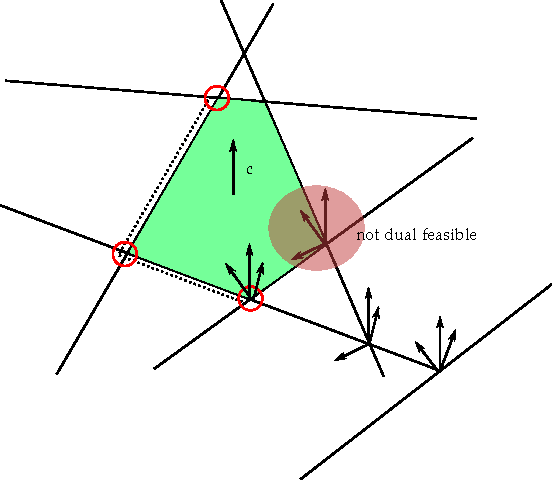
\includegraphics{./images/dualSimplex.pdf}
\end{center}
\caption{Dual Simplex}
\label{Fig:dualSimplex}
\end{figure}

We still keep a basis $B$ and $x_B=A_B^{-1}b$ but $x_B$ need not be positive anymore. Third we keep $\trans y=c_BA_B^{-1}$ and then we work towards a feasible primal solution. $\trans y$ should be feasible so 

\[\trans y A \leq c \quad 0 \leq c-c_BA_B^{-1}A \quad 0\leq \bar c\]

Assume we have a dual feasible basis $B$. Our tableau looks like this:

\begin{center}
\begin{tabular}{c|c}
$-c_Bx_B$ & $\bar c = c-c_BA_B^{-1}A$\\\hline
$A_B^{-1}x_B$ & $A_B^{-1}A$ %TODO is there a A_B^{-1} in the first column?
\end{tabular}
\end{center}

We know $\bar c = c-c_BA_B^{-1}A \geq 0$. If $x_B$ is positive, we're done. Otherwise there is some $x_{b_i}$ that is negative. We now kick out that index and bring in another one. Since we want to keep the costs greater than 0 we want to add a positive multiple $\Theta > 0$ of row $x_{b_i}$ to the cost vector, because there is a 1 in column $x_{b_i}$. That means we need

\[\bar c_k + \Theta v_k \geq 0,\quad \forall k\]

Where $v_k$ is the entry in ($x_{b_i}, k$). This is of course only interesting if $v_k<0$. We then need 

\[ \Theta \leq \frac{\bar c_k}{|v_k|} \quad \forall k\]

So we look for a column $j$ such that $v_j<0$ and 

\[j = \argmin{i} \frac{c_i}{|v_i|}\]

It can of course happen that all $v_k$ are greater than zero. Then the dual is unbounded, which means that the primal is infeasible. For a proof suppose the primal is feasible

\[\exists x\geq 0: Ax=b\]

If we multiply both sides with the inverse of the basis matrix we get TODO.

\begin{lstlisting}
Dual-Simplex
keep B s.t. $\trans y = c_BA_B^{-1}$ is feasible
until $x_B = A_B^{-1}b \geq 0$
	pick $b_i \in B$ s.t. $x_{b_i} <0$
	let $x_{b_i},v_1, v_2 \ldots, v_n$ be the row in the tableau
	if $v_k \geq 0\ \forall k$
		return Infeasible
	find j s.t. $v_j<0$ and $\bar c_j/|v_j|$ is minimal
	B = $B\backslash b_i \cup j$
return B
\end{lstlisting}

This algorithm can also be used to find an initial solution for the regular simplex algorithm. We can replace the cost vector by $0$ such that every feasible solution is optimal. We can then build the dual

\begin{align*}
\max \quad & \trans b y\\
s.t.\quad & \trans y A = 0\\
&y \text{ free}
\end{align*}

\marginpar{Lecture 11}
\section{Computational efficiency of Simplex}

We will examine the worst case running time, which will turn out to be exponential. Then we'll proceed to look at the average case running time, which is much better.

\subsection{Worst case}

\begin{Def} Let $T(I)$ be the running time of Simplex on instance $I\in \mathcal{I}(n,m)$. The worst case running time is defined as

\[\max_{I\in \mathcal{I}(n,m)} T(I)\]
\end{Def}

The running time per iteration is polynomial in $n,m$ (just matrix multiplications, something like O($n^3$)). The number of iterations is heavily dependend on the pivot-rule we choose (some pivot rules even have infinite running time in the worst case). However, for all know pivot rules there are examples for which the number of iterations is exponential.

These examples usually are based on the \emph{Klee-Minty-Cube}, which is a slightly altered multidimensional cube. We start with a normal multidimensional cube. A cube can be represented by $2n$ constraints and has $2^n$ vertices. As the next lemma shows there is a path that visits every vertex once.

\begin{lem} Every cube has a hamiltonian path, w.l.o.g. starting at $(0,\ldots,0)$\end{lem}

\begin{pr} By induction. For n=1 it's trivial. For $n\rightarrow n+1$ fix the first dimension and walk the path for $n-1$ dimensions. Then flip the fixed dimension and walk on the other cube. 

\[00\ldots0 \rightarrow 01\ldots0 \rightarrow 11\ldots 0 \rightarrow 10\ldots0\]
\end{pr}

To show that simplex actually is able to walk this path we need to find a corresponding cost vector. For example maximising $x_1$ would make simplex go directly to the destination, because that is the only edge that yields an improvement in the objective function. 

To avoid this uniquely determined edge this we perturb the cube slightly by adjusting 

\[0\leq x_1 \leq 1, \quad \epsilon x_{i-1} \leq x_1 \leq (1-\epsilon)x_{i-1}\]

This way there is more than one path that improves the cost. However, depending on the pivot rule we could still take the "right" edge and finish in one step. It is an important open question if there is a pivot rule such that simplex always needs less than exponentially many steps.

\subsection{Average Case}

Since Simplex is very fast in practice it's interesting to look at the average case. Since there is no natural probability distribution on linear programs we choose one distribution $f$. Then the expected running time is

\[\E_{I \stackrel{f}{\leftarrow}\mathcal{I}}[T(I)]\]

$f$ can be chosen for example like this: Given vectors $c$, $a_1,\ldots, a_m\in \R^n$ and scalars $b_1,\ldots b_m$ we introduce constraints of the usual form, either $\trans a_i x \leq b_i$, $\trans a_ix\geq b_i$, deciding between the possibilities by a coinflip. This of course produces $2^m$ linear programs, some of them feasible. It can be show that for such instances, under a fancy pivot rule, "shadow vertex", we need only linearly many iterations.

\begin{thm}[Haimich '83] Shadow vertex simplex requires at most $n/2$ iterations in expectation on a feasible input.\end{thm}

\subsection{Smoothed Analysis}

Another method for looking at the performance is a hybrid mix between worst-case and average-case analysis, the \emph{smoothed analysis}.

Given $I\\in \mathcal{n,m}$ we add random noise:

\[Ax\leq b \mapsto (A+\sigma G)x\leq b\]

Where $G$ is a matrix of random variables, choosen according to some probability distribution. $\sigma$ is a smoothening parameter that defines the size of the neighbourhood around a particular input in which we can run the algorithm. We call that neighbourhood $N(I,\sigma)$, the set of smoothed instances obtained from $I$. The smoothed running time is then the expected running time on the worst possible neigbourhood.

\[\max_{I\in \mathcal{n,m,}} \E_{J\stackrel{f}{\leftarrow} N(I,\sigma)} [T(J)]\]

By adjusting $\sigma$ you can choose between the worst case ($\sigma=0$), the average case ($\sigma = |I|$) and something in between.

You can show that the shadow vertex simplex algorithm has polynomial expected running time for $\sigma>0$ and $f$ a gaussian distribution.

\begin{thm}[Spielmann '01] For $f$= gaussian distribution, shadow vertex simplex runs in expected polynomial time for any fixed $\sigma>0$
\end{thm}

\subsection{Diameter of polytopes}

\begin{Def} The edge graph $G_p$ of a polytope is the graph made from the vertices of the polytopes. Edges are between adjacent vertices, i.e. two edges that are connected by a 1-dimensional face.
\end{Def}

\begin{Def} The distance between two vertices $x,y$, $d(x,y)$, is the length of the shortest path from $x$ to $y$ in $G_p$
\end{Def}

\begin{Def} The diameter of a graph is the maximum distance between two nodes\end{Def}

\begin{Def} Let $\Delta(n,m)$ be the maximum diameter of a polytope of size $n,m$

\[\Delta(n,m) = \max_{{P\in \R^n}\atop {m \text{ constraints}}} \text{diam}(P) \]
\end{Def}

$\Delta$ is a lower bound for the running time of simplex, as even the optimal way to switch bases needs to travel the whole diameter in the worst case. So if we want any chance of finding a polynomial pivoting rule we should first show that $\Delta(n,m)$ doesn't grow exponentially in $n,m$. 

\begin{thm}[Hirsch conjecture] $\Delta(n,m)\leq m-n$\end{thm}
\begin{thm}[Weak Hirsch conj] $\Delta(n,m)\leq \text{poly}(n,m)$\end{thm}

For unbounded polytopes the Hirsch conjecture has been disproven by a counterexample, but we still don't know if $\Delta$ grows polynomially or not.

It has however been show recently that 

\[\Delta(n,m)<m^{1+\log n}\]

It is not known whether the Hirsch conjecture is true in general, but we know some restricted polytope classes for which it holds, e.g. the assignment polytope from section \label{sec:maxAssignment} or any other perfect matching polytopes.

\subsection{Perfect matchings}

Perfect matching polytopes are defined as

\[P(G) = \text{conv} \{x(M) |M \text{ is perfect matching in }G\}\]

We can write that with constraints like this:

\begin{align*}
x_e \geq 0 &&\forall e\in E\\
\sum_{e=(u,v)} x_e = 1 &&\forall v\in V\\
\sum_{e\in E[S]} x_e \leq \frac{|S|-1}{2} &&S\subset V, |S| \text{ odd}
\end{align*}

\begin{thm} P defines the perfect matching polytope.\end{thm}
\begin{thm} For bipartite graphs the first two inequalities are enough to define the perfect matching polytope\end{thm}

Now we want to bound the diameter of perfect matching polytopes. Given perfect matchings $M,N$ let $x^M,x^N$ be the indicende vectors that define the vertices of the polytope

\begin{lem} $x^M$ and $x^N$ are adjacent iff $M\Delta N$ (the symmetric difference) is a circuit.\end{lem}

\begin{pr} $\Rightarrow$ $M\Delta N = \{C_1,\ldots, C_k\}$ circuits. If $k=1$ we're done. Otherwise we construct new perfect matchings $M'=M\Delta C_1$ and $N'=N\Delta C_1$. This does not affect the sum of the incidence vectors $x^M+x^N=x^{M'} +x^{N'}$. That means the convex combinations stay the same. But this is a contradiction to the assumption that $x^M$ and $x^N$ are adjacent vertices.

$\Leftarrow$ Define a weight function like this

\[w:\R \rightarrow \R \quad w_e=\begin{cases}0 & e\in M\cup N\\ 1 &\text{else}\end{cases}\]

This weight function has exactly two matchings of minimum costs, which must be adjacent
\end{pr}


\marginpar{Lecture 12}
\section{Implementation of the Simplex Method}

There are already many sophisticated simplex solvers, both free and commercial. Feasible problem sizes are in the order of a million variables and a million contraints (but with sparse constraints). 

Of course all implementations use floating point numbers and hence a subject to numerical instabilities. 

We already know the tableau method, cf. section \ref{sec:tableau}. The greatest drawback of this method is that the tableau matrix $A_B^{-1}A$ is usually a dense matrix (even when $A$ is sparse) so that the updates and the storage costs are very expensive.

\subsection{Revised simplex}

To carry out one iteration we only need the column that enters the basis, the inverse of the basis matrix $A_B^{-1}$ and the cost vector. In the normal tableau method we keep all the columns, now we recompute the column, when we need it.

\begin{lstlisting}
$x_B$ = $A_B^{-1}b$
$\bar c = c-c_BA_B^{-1}A$
select entering variable $j$ by looking at $\bar c$
compute $(A_B^{-1}A)_j = A_B^{-1}A_j$
select leaving variable $b_i$
move to basis $B\backslash b_i \cup j$ (update $A_B^{-1}$)
\end{lstlisting}

In the section about the tableau method we already saw that updating the inverse is easy, i.e. takes only quadratic many steps, instead of cubic for a full inversion. %If we want to add $\left(f\atop g)$ to $A_B$ we first compute \[A_B^{-1} \left(f\atop g\right) = \left(\tilde f \tilde g\right)\]

The other steps are easy too, so each step takes $O(m^2)$ and storage costs $O(m^2)$ for $A_B^{-1}$. The inverse of the basis matrix is still dense however.

\subsection{Sparse revised simplex}

We now improve the method to exploit sparse matrices. A sparse matrix has only "a few" nonzero entries in every row and column. The idea is to store only those instead of the whole matrix. For every row and column we store the nonzero elements and their respective index with the element. So every nonzero entry occurs in two linked lists. That reduced the storage costs of course, but makes random access on the matrix entries slower. Luckily we don't do random access during matrix multiplication, but we need the vector as an array. 

By this method we can compute $Ab$ in time proportional to the number of nonzero elements $\nz(A)$ in the matrix.

We also need the LU-decomposition. That means we factor a matrix $A$ into a lower diagonal matrix $L$ and a upper diagonal matrix $U$ such that $A=LU$. If we want it to be unique we force the diagonal of $L$ or the diagonal of $U$ to be 1. It can be computed by gaussian elimination, similar to the computation of the inverse. If you stop after half the steps you get the decomposition. The LU-decomposition of a sparse matrix frequently leads to sparse factors (in contrast to the inverse). However to get sparse $L,U$ some clever row or column permutation. We want to choose pivots that are not too small (for numerical reasons) and the product of the number of nonzero elements in the row and the column is small (Markowitz criterion).

Having an $LU$ decomposition is as good as having an inverse. Instead of solving $Ax=b$ we can solve

\[Ly=b\qquad Ux_B=y\]

But since $L,U$ are lower/upper diagonal we can simply solve those equations by backwards/forwards substitution. Again we only pay for the number of nonzero entries. The same technique can be applied to the other steps in the algorithm.

We have to think about how to update the $LU$ decomposition in each iteration.

Observe that $Ae_j\trans e_j$ is the matrix which is all zero except for the $j$th column which is identical to $A_j$. So switching a column can be written as

\[A_B-A_Be_{b_i}\trans e_{b_i} + A_j\trans e_j =A_B^{\text{new}} = A_B+(A_j-A_Be_{b_i})\trans e_j\]

We can now multiply this equation by $L^{-1}$ from the let where $A_B=LU$

\begin{align*}
L^{-1}A_B^{\text{new}} &= L^{-1}A_B+(L^{-1}A_j - L^{-1}A_Be_{b_i})\trans e\\
&= U+(\tilde A_j - Ue_{b_i})\trans e
\end{align*}

Which is $U$ with the $j$-th column replaced by $\tilde A_j$. We can compute a new $LU$ of the RHS\footnote{There is a lot of research how to do that cleverly.}, $\tilde L \tilde U$ the new $LU$ decomposition is then

\[A_B^{\text{new}} = L\tilde L \tilde U\]

But instead of computing $L\tilde L$ we keep the factorisation (which becomes more and more complicated) for a while until it is worthwhile to compute a fresh $LU$-decomposition directly from $A_B$.

\subsection{Exact solving}

In principle it's easy if the starting LP has rational coefficients. We just do rational arithmetic. It's awefully slow though. 

So to improve the runtime we run a fast floating point solver first and use the basis it returns as optimal as a starting basis. Usually the optimal basis should be very good so that we usually only need very few iterations to get to the actual optimal solutions.

Instead of switching to rational arithmetic immediately one can also increase the precision of the floating point arithmetic until that doesn't buy anything and then convert the solution to rational (with small denominators) by continued fraction expansion. Then do a few rational pivots if necessary.

It's an interesting research problem to define a suitable distance function between bases such that the runtime is proportional to the "quality" of the starting basis. This already works if the "good" basis is primal or dual feasible, but we don't know what to do for infeasible bases.

\marginpar{Lecture 13}
\chapter{Polynomial Methods for Linear Program Solving}

\section{The Ellipsoid Method}

Discovered by \href{http://en.wikipedia.org/wiki/Leonid\_Khachiyan}{Khachiyan} in 1979 it was the first method to show that Linear Programs can be solved in polynomial time. It is unique because it doesn't look at unnecessary constraints and makes it possible to solve some LPs with an exponential number of constraints in polynomial time. In practice it isn't used though, because it is very slow compared to the simplex method.

We'll only show how to solve feasibility, but it is easy to optimise once you can decide feasibility.

\[\{x|Ax\leq b\} = \emptyset?\]

Since the ellpsoid method works with volumes we'll have to make the assumption that either there is no feasible point at all or the set of feasible points has nonzero volume. More precisely we need that the set of feasible points in the ball with radius $4^{nL}$, centered at the origin, has volume at least $2^{-(n+1)L}$. $L$ is defined as 

\[L=n(1+\log C+\log n)\]

and the entries of $A,b$ are bound from above by $C$. This is basically the amount of bits you need to write down the problem description. These numbers may seem a bit magic, but they are needed to prove the polynomial runtime of the method.

It is possible to transform LPs with just a feasible point such that we get this nonempty volume without making infeasible problems feasible, by wiggling the constraints a bit.

Let $S$ be the set of feasible points inside the $n$-dimensional ball of radius $4^{nL}$ centered at the origin. The ellipsoid method maintains an ellipsoid $E$ that contains $S$. We check if the center of the ellipsoid is contained in the feasible region, if yes we're done, else there has to be some constraint that is violated there. We move the constraint to the center and construct a new ellipsoid that contains the half ellipsoid that is "more feasible". See figure \ref{Fig:ellipsoidMovement}.

The central result will be that the volumes of the ellipsoids decreases exponentially.

\begin{figure}[hbt]
\begin{center}
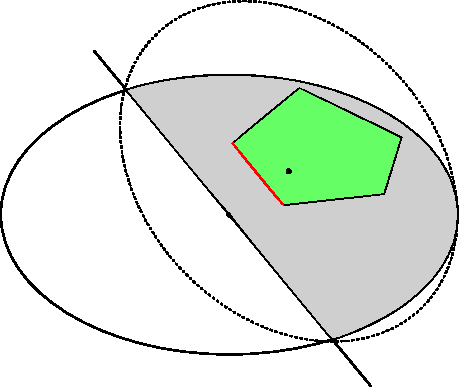
\includegraphics{./images/ellipsoid}
\end{center}
\caption{The final step of the ellipsoid method}
\label{Fig:ellipsoidMovement}
\end{figure}

In pseudocode the algorithm like as follows:

\begin{lstlisting}
E = ball of radius $4^{nL}$ centered at origin
while vol(E) $\geq 2^{-(n+1)L}$
	z = center of E
	if z is feasible return "feasible"
	let $\trans a_ix\leq b_i$ be a violated inequality
	//$\forall x\in S: \trans a_ix\leq b_i \leq \trans a_i z$
	let $1/2E = E\cap \{x|\trans a_i x \leq \trans a_iz\}$
	replace E by the smallest ellipsoid containing $1/2E$
return "infeasible"
\end{lstlisting}

$1/2E$ is the gray area in figure \ref{Fig:ellipsoidMovement}. The problem is how to find the ellipsoid that contains $1/2E$. 

\begin{Def}[Ellipsoid] An ellipsoid with center $z$ is defined as

\[E=\{x|\trans{(x-z)}Q(x-z)\leq 1\}\]

where $Q$ is a positive definite matrix, i.e. $\trans y Q y>0$ except for $y=0$.
\end{Def}

A simpler special case occurs if the initial ellipsoid is the unit ball and the violated constraint is parallel to a coordinate axis. See figure \ref{Fig:ellipsoidStart}

\begin{figure}[hbt]
\begin{center}
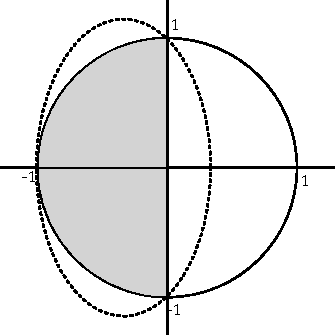
\includegraphics{./images/ellipsoidStart}
\end{center}
\caption{A simpler special case}
\label{Fig:ellipsoidStart}
\end{figure}

\begin{lem} Let $E$ be the unit ball, i.e. $E=\{x|\sum x_i^2\leq 1\}$. Then the smallest ellipsoid that contains $1/2E$, call it $\tilde E$ is

\begin{enumerate}
\item  We want to contain the halfball in an ellipsoid
\[\frac{1}{2}E=E\cap \{x|x_1\leq 0\} \subset \tilde E\]

Where $\tilde E$ can be computed like this
\[\tilde E = \left\{x\left|\left(\frac{n+1}{n}\right)^2\left(x_1+\frac{1}{n+1}\right)^2+\left(\frac{n^2-1}{n^2}\right) \sum_{i=2}^n x_i^2 \leq 1\right.\right\}\]
\item Also the volume of the new ellipsoid decreases.

\[\frac{vol(E')}{vol(E)}\leq f = e^{-1/2n}<1\]
\end{enumerate}
\end{lem}

\begin{pr} The funny terms in the definition of $\tilde E$ come from the case distinction: (1) $x_1=0$ and $\sum_i x_i=1$ (the intersection with the $y$-axis in figure \ref{Fig:ellipsoidStart}) and (2) $x_1=-1$, $x_i=0$. In both cases we want the inequality to be tight. It is easy to verify

\[\left(\frac{n+1}{n}\right)^2\left(0+\frac{1}{n+1}\right)^2+\left(\frac{n^2-1}{n^2}\right) = 1\]

and

\[\left(\frac{n+1}{n}\right)^2\left(-1+\frac{1}{n+1}\right)^2 = 1\]

In the general case the calculation gets more complicated.

Let $x$ be such that $\sum x_i^2\leq 1, -1\leq x_1\leq 0$. We show $x\in E'$
\[\frac{1}{n^2} \left( \underbrace{(n+1)^2}_{n^2+2n+1=n^2-1+2n+2} \left(x_1^2 + \frac{2}{n+1} x_1 + \frac{1}{(n+1)^2}\right) + (n^2-1)\sum_{i=2}^n x_i^2 \right)\]

\begin{align*}
\quad &= \frac{1}{n^2} \left((2n+2)x_1^2 + (2n+2)x_1+1+(n^2-1)\underbrace{\sum_{i=1}^n x_i^2}_{\leq 1} \right)\\
\quad &\leq 1+\frac{1}{n^2}(2n+2)\underbrace{x_1}_{-1\leq x_i\leq 0}(1+\underbrace{x_1}_{\geq -1})\\
\quad &\leq 1
\end{align*}

To prove the part about the volume we first need to recall that the volume of an ellipsiod is proportional to the length if its axes. $E$ has $n$ axes of length $1$, $E'$ has one axis of length $n/n+1$ and $n-1$ axes of length $\sqrt(n^2/n^2-1)$. So it decreases in one dimension, but grows in all the other dimensions. It is nontrivial to show that it shrinks in volume.

%TODO more comments, break in smaller parts
\begin{align*}\frac{vol(E')}{vol(E)}&=\frac{n}{n+1}\cdot \left(\frac{n^2}{n^2-1}\right)^{(n-1)/2}\\
&= \frac{n}{n+1}\cdot \sqrt{\frac{n^2-1}{n^2}} \cdot \left(\frac{n^2}{n^2-1}\right)^{n/2}\\
&=\sqrt{\frac{n^2-1}{(n+1)^2}} \left(\frac{n^2}{n^2-1}\right)^{n/2}\\
&=\sqrt{\frac{(n-1)(n+1)}{(n+1)^2}} \left(\frac{n^2-1+1}{n^2-1}\right)^{n/2}\\
\intertext{It is often helpful to rewrite things as exponentials, because we can bound logarithms more easily:}
&= \sqrt{\frac{n-1}{n+1}} \cdot \exp\left(\frac{n}{2} \ln (1+\frac{1}{n^2-1})\right)\\
\intertext{Now we use the fact that $\ln (1+x)\leq x$ for all $x>0$}
&\leq \sqrt{\frac{n-1}{n+1}} \cdot \exp\left(\frac{n}{2} \cdot \frac{1}{n^2-1}\right)\\
\intertext{We bound $1/(2n-1/n)$ by $1/(2n-1/2)$}
&\leq \sqrt{\frac{n-1}{n+1}} \cdot \exp\left(\frac{1}{2(n-1)}\right)\\
\intertext{Rewrite $n-1$ as $(n+1)-2$}
&=\sqrt{1-\frac{2}{n+1}}\cdot \exp\left(\frac{1}{2(n-1)}\right)\\
\intertext{Write everything as exponentials again to get rid of the squareroot}
&= \exp \left(\ln\left(\sqrt{1-\frac{2}{n+1}}\right)+\frac{1}{2(n-1)}\right)\\
&=\exp \left(\frac{1}{2}\ln \left(1-\frac{2}{n+1}\right) +\frac{1}{2(n+1)}\right)\\
\intertext{Use the trick for the logarithms from above}
&\leq \exp \left(\frac{1}{2} \cdot \frac{-2}{n+1} + \frac{1}{2(n-1)}\right)\\
&= \exp \left(-\frac{1}{n+1}+\frac{1}{2(n-1)}\right)\\
&\approx \exp \left(-\frac{1}{2n}\right)
\end{align*}

So we get

\[f \approx \exp \left(-\frac{1}{2n}\right)\]

\end{pr}

So in the special case for the unit ball we know that the volume decreases as we want.

In the General Case we intersect with a half space $H$ that contains the center $z$ of $E$ in its boundary. We will reduce it to the special case we just proved by

\begin{enumerate}
\item move $z$ to the origin
\[\trans{(x-z)}Q(x-z) \rightsquigarrow \trans xQx\]
\item rotate space such that axes of $E$ align with a coordinate axis. 

For this you need to find the eigenvectors of $Q$, as they are the axes of the ellipsoid. Then you can find their angle with the coordinate axes and use the appropriate \href{http://en.wikipedia.org/wiki/Rotation\_matrix}{rotation matrix}
\item scale the coordinates such that $E$ becomes the unit ball.

Since you already have the eigenvectors at hand from the previous step, calculate their length and scale everything accordingly using a \href{http://en.wikipedia.org/wiki/Scaling\_matrix}{scaling matrix}. This is easy because the axes are parallel to the coordinate axes after the rotation.
\item rotate it again such that $H$ becomes parallel to a coordinate axis
\item compute $E'$
\item reverse back to the original space by doing the transformations backwards.
\end{enumerate}

These steps change the volume of $E$ but they also scale the new ellipsoid $E'$ so that the relative volume of the two doesn't change.

So we proved that the volume of the ellipsoid shrinks by a factor in every step. After $k$ iterations $vol(E)$ is less than $f^k$ times the volume of the initial ball. The initial ball is contained in a cube with side length $2\cdot 4^{nL}$

\[vol(\text{cube}) = (2 \cdot 4^{nL})^n \leq 8^{n^2L}\]

If the $k$th iteration was not the last, i.e. we enter the loop body once more. Then $vol(E)$ must be

\begin{align*}
&2^{-(n+1)L} \leq vol(E) \leq f^k 8^{n^2L} \\
\Leftrightarrow & -(n+1)L  \leq k\log f + 3n^2 L && \log f \approx -\frac{1}{2n}\\
\Leftrightarrow & \frac{k}{2n} \leq (n+1)L+3n^2L \
\&Rightarrow k = O(n^3L)
\end{align*}

It could be that the real arithmetic we assumed could be exponentially expensive, but since $f$ is fairly far away from $1$ we can round a bit and turn the algorithm to a floating point version.

\begin{Ex}[Travelling Salesman Problem] We're going to formulate the problem as a ILP. For every edge $e$ we have a variable $x_e\in \{0,1\}$. An $x_e$ is $1$ if the corresponding edge is in the tour, $0$ else.

\begin{align*}
\min \quad & \sum_{e\in E} c_e x_e\\
s.t. & \sum_{e\in \delta(v)} x_e = 2 && \forall v\in V\\
	& \sum_{e\in S} \geq 2 && \forall S\neq V, S\neq \emptyset
\end{align*}
\[\delta(v) = \text{set of incident edges to $v$} \qquad \delta(S) = \text{edges with exactly one endpoint in $S$}, S\subseteq V\]

We can relax the problem to $0\leq x_1 \leq 1$ but there still are too many constraints to write the LP down. Using the ellipsoid method however we don't need to have all constraints given at any time. We just have to check whether some constraint is violated and if yes which one. We can check that by solving a mincut problem.
\end{Ex}

\marginpar{Lecture 16}
\section{The Interior Point Method}

This method was invented by Karmakar in 1984 and is a polynomial time method that is also fast in practice.

We're dealing with maximisation problems. Introduce some notation:

\[f_0(x) = cx,\quad f_i(x)=b-\trans a_i x\]

where $\trans a_i$ is the i-th row of A. Then we can write the feasible region like this

\[P=\{x|Ax\leq b\}=\{x|\forall i:f_i(x)\geq 0\}\]

Let $x^*$ be the optimal feasible solution and $p^*=cx^*$ the optimal objective value. 

Contrary to the simplex method we don't start at a vertex and walk around the boundary of the polyhedron, the interior points method starts in the interior and walks around the interior.

It works by turning constraints into penalties in the objective function (cf duals). 

\[t\in \R^+:\qquad g_t(x)=cx+\frac 1t \sum_{i=1}^m\ln (b_i-\trans a_i x)\]

The function $g_t$, although it looks complicated, is geometrically simple, as it is a stricly concave function. Finding maxima of concave functions is simple, $x^*(t)$, the maximiser of $g_t$ is easy to find and also unique. To find the unique maximum of $g_t$ we look at the partial derivative.

We will determine $x^*(t)$ for increasingly large values of $t$ by using the Newton method. From an approximate solution $x_0$ we take the first and second derivative at that point and compute the exact maximiser for the second order \href{http://en.wikipedia.org/wiki/Taylor\_expansion}{taylor approximation} of $g_t$. In two dimensions it would look like this:

\[q(x_0+h) = g_t(x_0) + h \cdot g_t'(x_0) + h^2 g_t''(x_0)/2\]

Maximising is easy, just write down the derivative and solve for h:

\[h = - \frac{g_t'(x_0)}{g_t''(x_0)} \]

In more dimensions we get the gradient vector of partial derivatives and the \href{http://en.wikipedia.org/wiki/Hessian\_matrix}{hessian matrix}. To ensure that we can find the maximiser we need to prove that the hessian looks nice. We'll do that later.

By iterating that process we can improve our solutions.

For $t\rightarrow \infty$, $x^*(t)$ converges to $x^*$. In fact we will prove:

\[cx^* -m/t \leq cx^*(t) \leq cx^*\]

where $m$ is the number of constraints. Also we have that a good approximation $x^*(t)$ is also reasonably good for $x^*(\mu t)$, for small $\mu$.

The value $(b_i-\trans a_i x)$ is positive for points in the interior of the polyhedron. The closer to the boundary we get the more negative $\ln (b_i-\trans a_i x)$ gets. So the sum gets very negative at the boundary. The $1/t$ factor dampens this influence so that we can get closer to the optimal solution (that has to lie on a boundary).

Let $\Phi(x)$ be defined as

\[\Phi(x) = \sum_{i=1}^m \ln (b_i-\trans a_ix) = \ln \prod_{i=1}^m (b_i-\trans a_i x)\]

$\Phi$ is called a logarithmic barrier function in the literature. Let's look at the level function of this barrier function, i.e. all the points where the value of the barrier function is constant

\[L_C=\{x|\Phi(x)=C\}\]

%pic

$L_C$ is a convex surface that is contained in the interior of $P$. Inside the curve $\Phi(x)>C$ outside it gets smaller. $L_C$ converges against the boundary of $P$ for $C\rightarrow -\infty$. %claim 4

So in conclusion the algorithm looks like this

\begin{lstlisting}
find $x^*(1)$ // by magic
while $t/m>\epsilon$ do
	$t = t\mu$
	find $x^*(t)$ from $x^*(t/m)$ by Newton
\end{lstlisting}

We prove the claim that $\Phi(x)$ is strictly concave. For two $x_0,x_1\in L_C$ and

\[x=\alpha x_0+(1-\alpha)x_1S\]

we have $\Phi(x)\geq C$ with equality only for $\alpha=0, \alpha=1$.

\begin{align*}
\Phi(x) &= \sum_{i=1}^m\ln (b_i - \trans a_i (\alpha x_0+(1-\alpha)x_1)\\
	&= \sum_{i=1}^m\ln (\alpha\underbrace{(b_i-\trans a_i x_0)}_r +(1-\alpha) \underbrace{(b_i-\trans a_i x_1)}_s)\\
	&\geq \alpha \sum_{i=1}^m \ln (b_i-\trans a_i x_0) + (1-\alpha)\sum_{i=1}^m \ln (b_i-\trans a_i x_1)\\
	&=\alpha C +(1-\alpha)C = C
\end{align*}

The $\geq$ holds because $\ln$ is concave and we have

\[\ln (\alpha s+(1-\alpha)r) \geq \alpha \ln s + (1-\alpha) \ln r\]

Since $cx$ is concave the sum of the two is also strictly concave. So $g_t$ has indeed a unique maximum. The maximiser $x^*(t)$ is a zero of the gradient (i.e. the vector of partial derivatives).

When $g_t$ is

\[g_t(x) = \sum_{i=1}^n c_i x_i + \frac{1}{t}\sum_{i=1}^m\ln (b_i-\sum_{j=1}^n a_{ij} x_j)\]

then the partial derivative with respect to $x_j$ is 

\[\frac{\partial g_t}{\partial x_j} = c_j+\frac 1t\sum_{i=1}^m \frac{-a_{ij}}{b_i-\trans a_i x}\]

So we can write the vector of partial derivatives as 

\[\frac{\partial g_t}{\partial x} = c-\frac{1}{t} \sum_{i=1}^m \frac{a_i}{b_i-\trans a_i x}\]

At $x^*(t)$ that vector is $0$. So at that point $c$ is a linear combination of the columns of the matrix (cf. duality).

Next we prove the claim that $c x^*(t) \geq p^*-m/t$. Look at the function

\begin{align*}
L(X) &= cx+\frac 1t\sum_{i=1}^m \frac{b_i-\trans a_i x}{b_i-\trans a_i x^*(t)}\\
\intertext{This function is not only linear in $x$, it is even constant}
 &= \frac 1t \sum_{i=1}^m \frac{b_i}{b_i- \trans a_i x^*(t) }+ \left(c + \frac 1t \sum_{i=1}^m \frac{\trans -a_i}{b_i - \trans a_i x^*(t)}\right)x
\end{align*}

Since the second term is the gradient of $g_t$ at $x^*(t)$ it is $0$ and $L(X)$ is constant.

We want to argue that the objective value at $x^*$ is less than $L(X)$

\begin{align*}
c x^* & \leq c x^* + \frac 1t \sum_{i=1}^m \frac{b_i-\trans a_i x^*}{b_i - \trans a_i x^*(t)}
\intertext{The fraction is $\geq 0$ since $x^*$ and $x^*(t)$ are feasible}
 &= L(x^*) && \text{by def.}\\
 &= L(x^*(t)) && \text{constant function}\\
 &= c x^*(t) + \frac 1t \sum_{i=1}^m \frac{b_i - \trans a_i x^*(t)}{b_i-\trans a_i x^*(t)}\\
 &=cx^*(t) + \frac mt
\end{align*}

We still have to argue that the hessian of $g_t$ looks good. The gradient was

\[\frac{\partial g_t}{\partial x} = c-\frac{1}{t} \sum_{i=1}^m \frac{a_i}{b_i-\trans a_i x}\]

Then the second derivative looks like this

\[\nabla g_t = \frac 1t  \sum_{i=1}^m \frac{a_{ij} - a_{ik} }{(b_i - \trans a_i x)^2}\]

So all the entries in the matrix are negative. It is formed by

\[-\frac{1}{t} \sum_{i=1}^m \frac{a_i}{b_i-\trans a_i x} \frac{\trans a_i}{b_i-\trans a_i x}\]

Hence we have 

\[\trans h H h = -\frac{1}{t} \sum_{i=1}^m\frac{\trans h a_i \trans a_i h}{(b_i - \trans a_i x)^2} \leq 0\]

and the hessian indeed describes a paraboloid.

\marginpar{Lecture 14}
\chapter{Integer Linear Programming}
\section{Introduction}

The setting is very similar to the linear programs we already know. We just restrict the problems and the possible solutions a bit. As the name suggests we want integer solutions to our programs. In general it is hard to tell whether some constraint system naturally describes a polyhedron where all optimal solutions are integral, so we need to actively restrict the solution space. 

\begin{Def}[Integer Linear Program] Given\footnote{In my oppinion $\R$ would be okay too} $A\in \Z^{m\times n}$, $b\in \Z^m$, $c\in \Z^{1\times n}$ find a $x\in \Z^n$ such that $Ax\leq b$ and $cx$ is maximal (or minimal)

\begin{align*}
\max \quad & cx \\
s.t. \quad & Ax \leq b\\
&x\in \Z^n
\end{align*}
\end{Def}

If we just restrict some variables to be integral and allow abitrary values for the others we have a mixed integer linear program.

Integer linear programs allow us to model some new interesting problems that we couldn't before. The most prominent examples are 

\begin{itemize}
\item binary choices, e.g. many NP-complete problems like Knapsack require some choice. 
\item relations between variables, e.g. choose at most ten of these things $\sum x_i \leq 10, x_i\in \{0,1\}$
\item disjunctive constraints, e.g. $x\geq a$ or $y\geq b$, can be modeled by introducing a decision variable $\delta \in \{0,1\}$ and saying $x\geq a\delta$ and $y \geq b(1-\delta)$. 
\item conditional constraints, e.g. if $x>a$ then $y>b$, can be modeled using disjunctive constraints: $x\leq a$ or $y>b$
\item piecewise linear cost functions become possible by introducing decision variables that decide on the piece we're in.
\end{itemize}

Integer Linear Programs are harder to solve than normal linear programs. Rounding, for example, doesn't work very well, as the cost difference between the optimal integral solution and an optimal fractional solution can be quite large.

\begin{thm} Finding a feasible solution for an ILP is NP-complete.
\end{thm}

\begin{pr} We prove by a reduction from SAT that ILP is NP-hard. For a given formula in CNF we construct an ILP like this:

For each variable $v_j$ in the formula we introduce $z_j \in \{0,1\}$ in our ILP, with the natural interpretation of the value of $z_j$. For every clause $C_i$ let $J^+_i$ be the number of positive and $J^-_i$ be the number of negated variables in clause $C_i$.

The ILP for the formula is then

\begin{align*}
\max \quad & 42 \\
s.t. &\sum_{j\in J^+_i} z_j + \sum_{j\in J^-_i} (1-z_j) \geq 1 && \forall i\\
&z_j \in \{0,1\}
\end{align*}

The constraints make sure that in every clause at least one positive variable is 1 or one negative variable is 0. If the feasible region of the LP is nonempty then the formula is satisfiable. The formal proof is omitted as it is rather obvious.

To show NP completeness we need to show that ILP is in NP. In the 0-1 case it is rather obvious that we can use any feasible solution as a polynomial witness. In the general case we would need to show that the entries in the solution vector are polynomially bounded. This is quite complicated but follows from the polynomial running time of the ellipsoid method. We will omit that proof here.
\end{pr}

NP-completeness is a worst-case statement. Some ILPs can be solved efficiently. We'll talk about conditions for that.

\section{Integer hull of a polyhedron}

The integer hull of a polyhedron is the set of feasible solutions $\{x | Ax\leq b, x\in \Z^n\}$. As we know $\{x|Ax\leq b\}$ is a polyhedron. Let $P_I = \{x| Ax\leq b\}_I$ be the convex hull of the integral vectors in $P$. See figure \ref{Fig:integerHull}

\begin{figure}[hbt]
\begin{center}
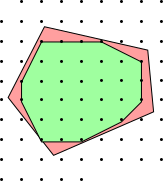
\includegraphics{./images/integerHull}
\end{center}
\caption{The integer hull of a polyhedron}
\label{Fig:integerHull}
\end{figure}

We make the following propositions:

\begin{enumerate}
\item If $P$ is bounded then so is $P_I$
\item If $A$ contains only rational numbers, $P$ is rational. For rational $P$ the integer hull is also a polyhedron.
\item If $P$ is unbounded and $A,b$ arbitrary real then $P_I$ is not necessarily a polyhedron.
\end{enumerate}

Obviously if $P=P_I$ then the solution for an ILP with feasible region $P_I$ is the same as the solution for the relaxed problem with feasible region $P$. This is the nice case where we can solve the ILP optimally in polynomial time using the methods we already know.

\begin{Def} A polyhedron $P$ is called integral if $P=P_I$\end{Def}

\begin{thm}\label{Thm:polyIntegrality} A rational polyhedron $P$ is integral iff

\[\max \{cx | x\in P\}\in \Z\quad \forall c\in \Z^{1\times n}\]

and the maximum is finite.
\end{thm}

\begin{pr} If the polyhedron is integral any optimal solution will also be integral, so that direction is easy.

For the other direction suppose $\max \{cx | x\in P\}\in \Z\quad \forall c\in \Z^{1\times n}$. Let $y\in P$ be a unique optimal solution for $c$. We have 

\[cy>cx + x_1 -y_1 \quad \forall x\in P,x\neq y\]

By multiplying $c$ be an arbitrary integer we can make the gap between the unique optimal solution $y$ and any other solution $x$ as large as we want, in particular large enough to make that inequality true.

We can change the cost function a bit without making $y$ nonoptimal. Let $\bar c = (c_1+1,c_{2,\ldots,n})$. We claim:

\[\bar c y > \bar c x\qquad \forall x\neq y\]

We want to compute by how much the cost changed. Since we increased the first component of $c$ we get

\[\bar c y = cy+y_1\]

Since we assumed that $cy$ is integral and our modification didn't impact integrality that equality forces $y_1$ to be integral too. We can do that for all components so they must all be integral. Since this must hold for all cost vectors it holds for all vertices and our polyhedron must be integral.
\end{pr}


\section{Total dual integrality}

As we said the case that $P=P_I$ is the nice case we can easily solve. In general it is hard to tell whether this is true, but for some constraint matrices we can prove that they always define integral polyhedra.

Strong duality as for linear programs does not hold for ILPs. But we have something similar

\begin{Def} A system $Ax\leq b$ is called totally dual integral (TDI) if for each integral $c$ with bounded maximum we have

\[\max \{cx |Ax\leq b\} = \min \{\trans y b | \trans y A = \trans c, y\geq 0, y\in \Z^m\}\]

Note that $x$ doesn't have to be integral here.

The same works for $Ax\leq b, x\geq 0$ and $Ax=b, x\geq 0$
\end{Def}

Notable here is that TDI is not a property of the polyhedron but instead of the system that defines it. Very much like with degeneracy we may find another system that describes the same polyhedron but is in fact TDI.

This together with theorem \ref{Thm:polyIntegrality} has the following corollary: Let $A\in \Q^{n\times m}$, $b\in \Z^n$ and $Ax\leq b$ is TDI then $\{x|Ax\leq b\}$ is integral.

This condition is checkable, but we don't really know how to use it yet.

\begin{Ex} Given a directed graph $G=(V,E)$, two vertices $s,t\in V$ and the set of pathes between $s,t$. We're also given a cost function $c$ on the edges. The task is to assign positive weights $y_e$ to the edges s.t. each path has accumulated cost at least 1. While doing so we want to minimize

\[\sum_{e\in E} c(e), y_e\]

Formulated as a LP that is 

\begin{align*}
\min \quad & \sum_{e\in E} c(e) y_e\\
s.t. & \sum_{e\in p} y_e \geq 1 && \forall p\in P\\
&y_e \geq 0
\end{align*}

We want to show that the polyhedron $Q$ that is defined be the above constraints is integral by showing that it is TDI. To do that we construct the dual:

\begin{align*}
\max \quad & \sum_{p\in P} x_p\\
s.t. & \sum_{p,e\in P} x_p \leq c(e) && \forall e\in E\\
 & x_p \geq 0 && p\in P
\end{align*}

By looking hard at the dual we see that it defines a maximum flow problem. As we know maximum flow problems with integer capacities have integral optimal solutions. Hence we have a TDI system.
\end{Ex}

\marginpar{Lecture 15}
\begin{thm} For each rational polyhedron, there exists a TDI system $Ax\leq b$ with an integral matrix $A$. {\small (no proof)}
\end{thm}

The most important aspect of TDIness is the following theorem

\begin{thm} If $Ax\leq b$ is TDI and $b$ is integral, then $P=\{x|Ax\leq b\}$ is integral.
\end{thm}

\begin{pr} The proof is by contradiction. Assume $P$ is not integral and take a fractional vertex $x$ of $P$. Construct an integral cost vector $c$ such that $x$ is optimal, by taking a rational one and scaling.

In particular that means if $b\in \Z$ then the whole polyhedron is integral.
\end{pr}

\section{Totally unimodular matrices}

TDIness is a little weird and hard to check. A much easier recognizable property that also implies integrality of the polyhedron is total unimodularity.

\begin{Def} A matrix $A$ is totally unimodular (TU) if each subdeterminant (the determinant of a square submatrix), i.e. each \href{http://en.wikipedia.org/wiki/Minor\_\%28linear\_algebra\%29}{minor}, of $A$ is $\in \{-1,0,1\}$
\end{Def}

That means in particular that also all entries are $\in \{-1,0,1\}$.

\begin{thm}[Hoffman, Kruskal '56] $A\in \Z^{m\times m}$ is TU iff $P=\{x|Ax\leq b\}$ is integral for any integral $b$
\end{thm}

\begin{pr} $\Rightarrow$ Let $A$ be TU, $b\in \Z^m$ and let $x$ be a vertex of the induced polyhedron $P$. $x$ is a solution of $A'x=b'$ with $A'x\leq b'$ being a subsystem of 

\[\left(A|-I\right) x \leq \left(b\atop 0\right)\]

with $A'$ being a non-singular submatrix. Since $A$ is TU we have $\det A'\in \{-1,1\}$. This already implies that the polyhedron is integral, because we can compute the inverse $A'^{-1}$ using Cramer's rule. %TODO


The following isn't completely correct yet:

$\Leftarrow$ Suppose all vertices of $P$ are integral vectors $\forall b\in \Z^m$. We want to show that every nonsingular square submatrix has a determinant of $\{1,-1\}$. By switching rows and columns around we can assume that the submatrix $A'$ lies in the topleft corner of $A$ (that only changes the sign of the determinant). 

We expand $A$ by the identity matrix, $(A|I)$. Then we can construct a new matrix $B\in \Z^{m\times m}$ such that $\det (A') = \det (B)$ by taking 

\[B = \left({A' \atop *} {0\atop I}\right)\]

To prove $|\det (B)| =1$ it suffices we show $B^{-1}$ is integral because

\[\det(B)*\det(B^{-1}) = 1\]

and our knowledge that $\det (B)$ is integral (since $B$ is integral). If $B^{-1}$ is also integral we multiply two integrals. We can only get $1$ if both are either $1$ or $-1$.

To prove $B^{-1}$ is integral we choose $i\in \{1,\ldots, m\}$ and show that $B^{-1}e_i\in \Z^m$. Take some $y\in \Z^m$ s.t. $z:= y + B^{-1}e_1\geq 0$. $z$ will later become the vertex of our polyhedron. 

By multiplying both sides with $B$ we get $b:= Bz=By+e_i$. $b$ is integral because $B$,$y$ and $e_i$ are integral. We can add $n$ zeros to the middle of $z$ such that the new $z'$ fulfills $(A|I)z'=b$. The first $n$ entries of $z'$, call them $z''$ is in $P$ since

\[Az''\leq b\]

In particular the $k$ constraints from $A'$ are fulfilled with equality because we know $(A|I)z'=b$. It also fulfils $m-k$ non-negativity constraints, so it's a vertex:

\[\begin{pmatrix}
A' & *\\
* & *\\
-I_k & 0 \\
0 & I_{m-k}
\end{pmatrix} \cdot z'' \leq \left(b \atop 0\right)\]

That means $z''$ is integral, because the polyhedron is integral. That implies that $z'$ is also integral, since $b$ is integral and the lower components are produced by the identity matrix. Then of course $z$ is also integral.

Then we have from the definitions above

\[z-y=B^{-1}e_i\]

But since $z$ and $y$ are integral $B^{-1}e_i$ must also be integral.

\end{pr}

\begin{thm} Let $A\in \Z^{m\times m}$. The following statements are equivalent
\begin{enumerate}
\item $A$ is TU
\item $\forall b \in \Z^m, c\in \Z^m$:
\[\max \{cx|Ax\leq b, x\geq 0\} = \min \{\trans y b|\trans A \geq c, y\geq 0\}\]
and they have integral optimal solutions or are unbounded
\item $Ax\leq b, x\geq 0$ is TDI for all $b\in \Z^m$
\item $\forall\ \text{rows}\ R\subset \{1,\ldots, m\} \exists\ \text{partition}\ R = R_1 \dot \cup R_2$ such that

\[\sum_{i\in R_1} a_{ij} - \sum_{i\in R_2} a_{ij} \in \{-1,0,1\}, \qquad \forall j\in \{1,\ldots, n\}\]
\end{enumerate}
\end{thm}

The last part tells us something about edge incidence matrices of graphs and total unimodularity: for all undirected graphs is totally unimodular iff the graph is bipartite. We can then partition the matrix like requested by using the two partitions of the graph. Then the difference must always be zero.

\marginpar{Lecture 17}
\begin{thm} Let $A\in \{0,1,-1\}^{m\times m}$, where each column has at most one $-1$ an at most one $1$ entry. Then $A$ is totally unimodular.
\end{thm}

\begin{pr} Let $N$ be a $k\times k$ submatrix of $A$. We do induction on $k$. For $k=1$ it's trivial.

Remember, determinants can be computed like this

\[\det A = \sum_{i=1}^n a_{ij} \cdot (-1)^{i+j} \det A_{ij} = \sum_{j=1}^n a_{ij} \cdot (-1)^{i+j} \det A_{ij}\]

There are two cases

\begin{itemize}
\item If $N$ has a column with at most one non-zero entry. We can just expand on that column to reduce the determinant of $N$ to the determinant of one $k-1\times k-1$ submatrix $N'$.

\item If all columns of $N$ have 2 non-zero entries (more are impossible by definition of $A$), the sum of all rows is $0$ so $N$ is singular and the determinant is $0$
\end{itemize}
\end{pr}

A nice corollary from this theorem is the fact that the node-edge incidence matrix (rows=vertices, columns=edges, $1$ if edge is at vertex) of any digraph is TU.

\chapter{Solving Integer Programs}
\section{Cutting Planes and Cutting Plane Algorithms}
In most cases the ployhedron we describe with our integer linear program is not nicely integral.

A cutting plane algorithm tries to cut off parts of the polyhedron that are not in the integer hull of the polyhedron.

The idea here is that it's easy to find the integer hull of a halfplane. 

\[\trans a x \leq b \quad \Rightarrow \quad \trans a x \leq \lfloor b \rfloor\]

where the inequality is scaled s.t. $a$ is integral and $\gcd(a)=1$. Rounding down the right hand side shifts the hyperplane such that it intersects with the closest feasible integer point.

We could to this transformation for every valid constraint for the polyhedron. However there are quite a few and we'd need to iterate the process because the new inequalities change the set of valid constraints.

Instead we just try to cut off things around the optimal solution until it becomes integral. That means we don't have to care about the other parts of the polyhedron and hopefully speeds up the process.

To find the right cutting planes we first solve the linear program relaxation to get some $x^*$. The we find some hyperplane that cuts off $x^*$ without touching the integer hull, i.e. it is valid for $P_I$, and add it to our LP.

\begin{lstlisting}
repeat
	$x^*$ = Solve LP $\max \{cx|x\in P\}$
	if $x^*$ is integral return $x^*$
	$H$ = halfspace that separates $x^*$ from $P_I$
	$P=P\cap H$
\end{lstlisting}

Of course we don't know how to find the cutting plane that cuts off $x^*$, or even how to check if a given inequality is valid for $P_I$. It's also not clear if this algorithm always terminates and if it terminates how long it takes.

\subsection{Cutting plane proofs}

There are many different ways to find cutting planes. In the following we will deal with Gomory-Chvatal cuts.

We want to prove that some inequality $\trans cx\leq \delta$ is valid for all integral solutions of $Ax\leq b$

\begin{Ex}
Let the system be

\[\begin{pmatrix}
2 & 3\\
2 & -2 \\
-6 & -2\\
-2 & -6\\
-6 & 8
\end{pmatrix}\cdot x \leq \begin{pmatrix} 27\\7\\-9\\-11\\21\end{pmatrix}\]

We look at linear combinations of the rows. For example we see by scaling rows 5:

\[-3x_1+4x_2 \leq \frac{21}{2}\]

This means we can round down $21/2$ to $10$ because $x_1,x_2$ are integral. From adding two times that new inequality to three times the first one we get

\[17x_2 \leq 101 \quad \Rightarrow \quad x_2 \leq \left\lfloor \frac{101}{17}\right\rfloor = 5\]
\end{Ex}

In general we want to find inequalities of the form

\[\trans y A x \leq \left\lfloor \trans y b \right \rfloor,\quad y\geq 0, \trans y A \text{ integral}\]

These inequalities are called Gomory-Chvatal cutting planes.

\begin{Def} Let $Ax\leq b$ system of $m$ linear inequations and $\trans cx\leq \delta$ an inequality. A sequence of linear inequalities $c_1x\leq \delta_1, c_2x\leq \delta_2,\ldots, c_mx\leq \delta_m$ is called a \emph{cuting plane proof} of $\trans c x\leq \delta$ from $Ax\leq b$ if
\begin{itemize}
\item $c_1,\ldots c_m$ are integral
\item $c_m=c$ and $\delta_m=\delta$
\item $\forall i\in [1,m]: c_ix\leq \delta_i'$ is a nonnegative linear combination of inequalities from the system

\[Ax\leq b, c_1x\leq \delta_1,\ldots,c_{i-1}x\leq \delta_{i-1}\]

and $\delta_i=\lfloor \delta_i'\rfloor$.
\end{itemize}
\end{Def}

\begin{thm}[Existence] Let $P=\{x\in \R^n | Ax\leq b\}$ be bounded and non-empty

\begin{enumerate}
\item if $P_I\neq \emptyset$ and some inequality $\trans c x\leq \delta$ with integral $c$ is valid, then there is a cutting plane proof
\item if $P_I=\emptyset$ then there is a cutting plane proof of 
\[0x\leq -1\]
\end{enumerate}
\end{thm}

\begin{thm}[Finite Length] Let $Ax\leq s$ be a rational system of linear inequalities with at least one integral solution If $\trans cx\leq \delta$ is valid for integral $c$, then $\trans cx\leq \delta$ has a cutting plane proof of finite length.
\end{thm}

While looking for Gomory-Chvatal cuts we usually use the cuts we already added to form new cuts. If we don't do that but instead add all cuts that we can form without taking into account the new constraints we form the Chvatal closure of the polyhedron.

\begin{Def} Let $P=\{x|Ax\leq b\}$ be a rational polyhedron. Adding all Gomory-Chvatal cuts $\trans yAx\leq \lfloor \trans y b\rfloor$ for $y\geq 0$ and $\trans y A$ integral, yields the \emph{Chvatal Closure}
\end{Def}

\begin{thm} The Chvatal Closure is a polyhedron\end{thm}

\marginpar{Lecture 18}
For TDI systems the cuts to form a Chv\'{a}tal closure are easy to characterise

\begin{thm} Let $P=\{x|Ax\leq b\}$ be a polyhedron with $Ax\leq b$ is TDI and $A$ integral. 

The Chv\'{a}tal closure is $P'=\{x|Ax\leq \lfloor b\rfloor\}$
\end{thm}

\begin{pr}[]For the case $P\neq \emptyset$. Let the Chv\'{a}tal closure be $C$

$C\subset \{x|Ax\leq \lfloor b\rfloor\}$. It is clear that rounding down the right sides constitutes a Gomory-Chv\'{a}tal cut. The closure may have some more, so it's smaller.

$\{x|Ax\leq \lfloor b\rfloor\} \subset C$. Let $y\geq 0$ such that $\trans y A$ is integral. We need to show 

\[\forall x: Ax\leq \lfloor b \rfloor: \trans y A \leq \lfloor \trans y b\rfloor\]

That means rounding down gives us the same solutions as we get by applying the definition of Chv\'{a}tal closure. To use TDIness we look at

\[\trans yb \stackrel{Ax\leq b}{\geq} \max \{\trans y Ax | Ax\leq b\} = \min \{\trans v b|v\geq 0, \trans v A = \trans y A\}\]

Since $\trans y A$ is integral and $Ax\leq b$ is TDI we know there is some integral optimal vector $v^*$ for the dual. We then get

\[\trans y A x =\trans {v^*} A x \stackrel{Ax\leq \lfloor b\rfloor}{\leq} \trans{v^*} \lfloor b\rfloor \leq \lfloor \trans{v^*} b\rfloor \leq \lfloor \trans y b\rfloor\]

Which proves the claim.
\qed \end{pr}

We know that every rational polyhedron (and every bounded polyhedron) has a minimal TDI system that defines it. We can then find the Chv\'{a}tal closure easily and get a new polyhedron, for which we can then again find a TDI description and repeat the procedure.

Unfortunately finding TDI descriptions is hard and the number of iterations can be arbitrarily large. The number of iterations of adding the Chv\'{a}tal closure until we get the integer hull is called the \emph{Chv\'{a}tal rank}.

\subsection{Gomory's cutting plane algorithm}

The idea is to run simplex and the look at the final tableau. Find some row with fractional result and round everything down. 

\[x_i + \sum_{j\in N} \bar a_{ij} x_j = \bar a_{i0} \quad \Rightarrow \quad x_i + \sum_{j\in N} \lfloor\bar a_{ij}\rfloor x_j = \lfloor\bar a_{i0}\rfloor\]

Add that as a new constraint and repeat. 

It is ok to round down the $\bar{a_{ij}}$ because $x\geq 0$ and rounding down makes everything smaller, so the inequality is still satisfied. Rounding down the $\bar a_{i0}$ is ok because that's just the Chv\'{a}tal cut.

The new constraint cuts off at least the optimal solution simplex found. This has the nice property that we don't add cuts in regions that aren't interesting to us.

\begin{Ex} Let the ILP we want to solve be
\begin{align*}
\min \quad& x_1-2x_2\\
s.t. \quad& -4x_1 +6x_2 \leq 9\\
& x_1+x_2 \leq 4
&x_1,x_2 \in \N
\end{align*}

The first solution we get with simplex is $x=(15/10,25/10)$. The interesting row in the tableau is

\[x_2+1/10 x_3 + 1/10x_4 = 25/10\]

We add the cut

\[x_2 \leq 2\]

With that constraint we get the solution $x=(3/4,2)$ with the following row in the tableau

\[x_1-1/4x_3 +6/4 x_5 = 3/4\]

We add the cut

\[x_1-x_3+x_5\leq 0\]

Because $x_3$ and $x_5$ are slack variables ($x_5$ is for the first cut), we can replace them 

\[x_5 = 2-x_2\qquad x_3=9+4x_1-6x_2\]

With these constraints we get an integral solution.
\end{Ex}

\begin{thm} Gomory's Algorithm terminates after a finite number of iterations, when it is using the lexicographic dual simplex.
\end{thm}

\marginpar{Lecture 19}
\subsection{Cuts for TSP}

Gomory's algorithm is a general method that works for any ILP. Creating the cuts doesn't assume anything about the combinatorial structure of the problem and hence often isn't optimal.

Here we want to show how to exploit the structure of a problem, the Travelling Salesman Problem, to find some cuts for the polyhedron.

We're given a graph $G=(V,E)$ and want to find a minimum cost tour. 

In the standard formulation that we've already seen we have a variable for each edge, indicating if the edge is in the tour.

\begin{align*}
\min \quad & \sum_{e\in E} x_e c_e\\
s.t.\quad & \sum_{e\in \delta(v)} x_e = 2 && \forall v\in V \quad \text{all nodes used}\\
	& \sum_{e\in E(S)} x_e \leq |S|-1 && \forall S\subset V, 2\leq |S| \leq |V-1| \quad \text{only one cycle}\\
	& x_e \in \{0,1\}
\end{align*}

As we already said this uses an exponential number of constraints, but we don't bother with that right now.

The cuts we will add use \emph{combs}

\begin{Def}[Comb] %pic
A comb with handle $H$ and teeth $T_1,\ldots T_k$ consists of node sets $H$ and $T_i$ such that $T_i \cap T_j = \emptyset$, $H\cap T_i\geq 1$ and $|T_i\backslash H |\geq 1$ and $k$ is $\geq 3$ and odd.
\end{Def}

\begin{figure}[hbt]
\begin{center}
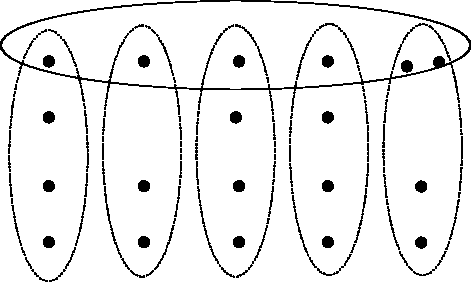
\includegraphics{./images/comb}
\end{center}
\caption{A comb in a graph}
\end{figure}

%If we have a comb in the graph no tour can exist in the graph.

\begin{thm} Let $c$ be a comb with handle $H$ and teeth $T_1,\ldots, T_k$. Then any tour satisfies the following inequality

\[\sum_{e\in E(H)} x_e +\sum_{i=1}^k\sum_{e\in E(T_i)} x_e \leq |H|+\sum_{i=1}^k(|T_i|-1)-\frac{k+1}{2}\]
\end{thm}

\begin{pr} To get the constraint from the theorem we take a linear combination of the constraints of the program and invoke the Chv\'{a}tal cut theorem.

Use

\begin{itemize}
\item Add the first constraint for all $v\in H$
\item Subtract the third inequality for (relaxed to $-x_e\leq 0$) for all $e\in \delta(H)\backslash X$ where $X$ are the edges that belong to a tooth
\item add the second constraint for all $T_i$
\item add the second constraint for all $T_i\backslash H$
\item add the second constraint for all $T_i \cap H$
\end{itemize}

The gets us the following equations

\begin{align*}
\sum_{v\in H}\sum_{e\in \delta(v)} x_e&=2|H|\\
-\sum_{v\in H} \sum_{e\in \delta(v) \backslash E(T_i)} x_e & \leq 0\\
+\sum_{i=1}^k \sum_{e\in E(T_i)} x_e &\leq \sum_{i=1}^k(|T_i|-1)\\
+\sum_{i=1}^k \sum_{e\in E(T_i\backslash H)} x_e &\leq \sum_{i=1}^k(|T_i\backslash H|-1)\\
+\sum_{i=1}^k \sum_{e\in E(T_i\cap H)} x_e &\leq \sum_{i=1}^k(|T_i\cap H|-1)\\
\end{align*}

Adding up the first two equations counts all the edges in the handle twice

\[2\sum_{e\in E(H)} x_e \leq 2|H|\]

The last two equations sum up to

\[\sum_{i=1}^k \sum_{e\in E(T_i)} x_e \leq \sum_{j=1}^k (|T_i|-1) -k\]

Summing up everything we get

\begin{align*}
2\sum_{e\in E(H)} x_e + 2\sum_{i=1}^k \sum_{e\in E(T_i)} x_e &\leq 2|H| + 2\sum_{j=1}^k (|T_i|-1) -k\\
\Leftrightarrow \sum_{e\in E(H)} x_e + \sum_{i=1}^k \sum_{e\in E(T_i)} x_e &\leq 2|H| + \sum_{j=1}^k (|T_i|-1) -\frac{k+1}{2}
\end{align*}

We replace $-k/2$ by $-(k+1)/2$ because $k$ is odd and we round everything down.
\qed \end{pr}

Unfortunately there are exponentially many comb cuts, and there is no polynomial algorithm to find one that is violated s.t. we might add it. There are however exponential time algorithms that find them and there are heuristic methods that sometimes find them.

So we can solve TSP by relaxing the LP. Usually we also drop the second constraint and allow more than one circle. We then try to find violated constraints. If we have more than one circle it's easy to find a violated constraint, else we have to find comb constraints either by the heuristic method or the exponential one. Should we be unable to find violated constraints although we don't have an integral solution yet, we need to use some other method like for example branch and bound.

\section{Branch and Bound}

With cutting plane algorithms we don't have any feasible solutions during the run of the algorithm, because we're solving relaxations all the time.

Branch and bound techniques actually work with feasible solutions that get improved iteratively. The approach is similar to divide-and conquer. We recursively partition the feasible region into sets and take the maximum (or the minimum) on it. That gives us a search tree of subproblems we need to solve. We use simplex or some other heuristic to find bounds on the optimal values such that we can cut off search paths that are not interesting.

There are some design choices we can make

\begin{itemize}
\item In what order to look at subproblems: DFS, BFS, Best-First, \ldots
\item How to compute bounds: LP relaxation, Lagragian relaxation (later), cutting planes
\end{itemize}

For general ILPs we can for example do the following: 

Use the LP relaxation for bounding. Branch by fixing components of the solution. For an optimal solution $x^*$ fix fractional values by adding constraints

\[x_i\leq  \lfloor x_i^*\rfloor \qquad x_i \geq \lceil x_i^* \rceil\]

\begin{Ex}[TSP] For the following relaxed formulation of the TSP

\begin{align*}
\min \quad & \sum_{i,j} c_{ij}x_{ij}\\
s.t. \quad & \sum_{j} x_{ij} = 1\\
	& \sum_{i} x_{ij} = 1\\
	& \sum_{ij\in S} x_{ij} \leq |S|-1 && S \subseteq \{1,\ldots,n\}, |S|\geq 2, |S| \leq |V|-1\\
	& x_{ij} \geq  0
\end{align*}

If we remove the constraint that forbids more than one circle we get the assignment problem (perfect matchings), which we can solve in polynomial time. We can use that as a bound for the TSP.

We branch by forbidding certain edges in the solution, i.e. we get some set of cycles from the relaxation, choose the shortest and create subproblems in which one of the edges on the cycle is fixed to 0.
\end{Ex}


%\marginpar{Lecture 19}
%\input{./lecture19}

\marginpar{Lecture 20}
\section{Langrangean Relaxation}

For an ILP we typically can separate the constraints in two classes, the hard constraints $A$ and the easy constraints $D$\footnote{TODO: switch A and D everywhere. D for difficult :/}. What hard and easy mean depends on the problem, but usually the problem would be solvable in polynomial time if it were not for the hard constraints.

The idea of langrangean relaxation is to relax the hard constraints, but  a penalty into the objective function for violating them.

For some $\lambda>0$

\begin{align*}
\max \quad & c x + \trans{\lambda}(b-Ax)\\
s.t. \quad & Dx \leq d\\
	& x\in \Z
\end{align*}

If we violated the $Ax\leq b$ constraints we subtract something from our objective value.

This is called the langrangean relaxation of the problem, the $\lambda_i$ are the Langrange multipliers.

Since we said that the constraints in $D$ are "easy" we assume that we can solve this problem in polynomial time for some fixed $\lambda$.

\begin{thm} Let $\lambda \geq 0$ and $z^*,z(\lambda)$ be optimal values of the ILP, LP$_\lambda$ respectively.

\begin{enumerate}
\item the feasible region of the ILP is smaller than the feasible region of LP$_\lambda$
\item $z(\lambda)\geq z^*$, i.e. the relaxed version gives us an upper bound on the optimal value.
\end{enumerate}
\end{thm}

\begin{pr} The first part is rather obvious, since we remove constraints the feasible region can only get larger.

For the second statement let $x^*$ be an optimal solution to the ILP. Since it's optimal it must also be feasible

\[Ax^*\leq b\]

But in the relaxed version we also have some additive Then we have

\[z(\lambda) \geq cx^* + \trans{\lambda}\underbrace{(b-Ax^*)}_{\geq 0} \geq cx^*=z^*\]
\qed \end{pr}

So this is a relaxation for every $\lambda$. But since we want to find upper bounds that are as tight as possible, we look for a $\lambda$ that minimises $z(\lambda)-z^*$. Because we know that $z(\lambda)\geq z^*$ for all $\lambda$ we can just minimise $z(\lambda)$. This is called the Langrangean Dual

\[z_{LD} = \min_{\lambda\geq 0} \{z(\lambda)\} = \min_{\lambda\geq 0} \max_{{x\in \Z}\atop {Dx\leq d}} cx+\trans{\lambda}(b-Ax) \]

For a discussion on how to actually find the optimal $\lambda$ see the book by Tsitsiklis and Bertsimas.

\subsection{Quality of the Langrangean}

We want to investigate how good the bounds are that we get out of the langrangean relaxation. First we observe that in some special cases the optimal value of the langrangian dual can be optimal for the ILP too.

\begin{thm}\label{thm:relaxedOptimal} Let $\lambda \geq 0 $ and let $x_\lambda$ be an optimal solution for the relaxed $LP_\lambda$. If we have

\begin{enumerate}
\item $Ax_\lambda \leq b$
\item $\trans{\lambda}(b-Ax_\lambda) = 0$
\end{enumerate}

then $x_\lambda$ is also an optimal solution for the ILP.
\end{thm}

\begin{pr} Let $x^*$ be an optimal solution to the ILP. By the first condition our penalty term $\trans{\lambda}(b-Ax_\lambda)$ is positive in every component, so for the optimal relaxed value we know: $z_\lambda ^*\geq c x^*$. Since by the second condition we know that the penalty is actually: $\trans{\lambda}(b-Ax_\lambda) = 0$, we know we have equality.

Note: we need the $Ax_\lambda \leq b$ condition because $\lambda$ could be 0.
\qed \end{pr}

Next we compare the quality of the langrangean relaxation with the easier linear programming relaxation.

\begin{thm} In general

\[z_{LD} \leq z_{LP}\]

Equality holds if the "easy" constraints describe an integral polyhedron.
\end{thm}

\begin{pr} By definition we have

\[z_{LD} = \min_{\lambda \geq 0} z(\lambda) = \min_{\lambda\geq 0} \max_{{x\in \Z}\atop {Dx\leq d}} z(\lambda,x)\]

If the polyhedron $Dx\leq d$ is integral we can just drop the integrality constraint on $x$, otherwise the solution might get better.

\[\min_{\lambda\geq 0} \max_{{x\in \Z}\atop {Dx\leq d}} z(\lambda,x) \geq \min_{\lambda\geq 0} \max_{Dx\leq d} z(\lambda,x)\]

With equality only in the case of integrality.

So we have

\begin{align*}
z_{LD} &\geq \min_{\lambda\geq 0} \max_{Dx\leq d} cx+ \trans{\lambda}(b-Ax)\\
	& = \min_{\lambda \geq 0} (\trans{\lambda}b+\max_{Dx\leq d}(c-\trans{\lambda}A)x)\\
\intertext{Now we dualise the last part. By strong duality the value does not change.}
	& = \min_{\lambda \geq 0} (\trans{\lambda} b+\min_{y\atop {\trans yD=c-\trans{\lambda}A}} \trans y d)\\
	&= \min_{{{\lambda \geq 0}\atop {y\geq 0}}\atop {\trans yD=c-\trans{\lambda}A}} \trans{\lambda} b+ \trans y d\\
	&=\max_{{Ax\leq b}\atop {Dx\leq d}} cx = z_{LP}
\end{align*}
\qed \end{pr}

\subsection{TSP --- Held-Karp-Bound}

We had the following ILP to solve the TSP.

\begin{align*}
\min \quad & \sum_{e\in E} c_{e}x_{e}\\
s.t. \quad & \sum_{e\in \delta(v)} x_{e} = 2 && \forall v\in V\\
	& \sum_{e\in E(S)} x_{e} \leq |S|-1 && S \subseteq \{1,\ldots,n\}, |S|\geq 2, |S| \leq |V|-1\\
	& x_{e} \geq  0
\end{align*}

We can add some redundant constraints without changing the solution

\begin{align*}
\min \quad & \sum_{e\in E} c_{e}x_{e}\\
s.t. \quad & \sum_{e\in E} x_e = n\\
	&\sum_{e\in \delta(v)} x_e=2 && \forall v=\{2,\ldots,n\}\\
	&\sum_{e\in \delta(1)} x_e=2\\
	&\sum_{e\in E(S)} x_e \leq |S|-1 && \forall S \subseteq V, 2\leq |S|\leq |V|-1,1\not i\in S\\
	& x_{e} \geq  0
\end{align*}

The second constraint in this program is the difficult one (as we'll see when we analyse the relaxed problem). We can form the lagrangean relaxation by takeing it into the cost function.

For any $\lambda$\footnote{for some reason it's ok to take negative $\lambda$ too\ldots}

\begin{align*}
\min \quad & \sum_{e\in E} c_e x_e + \sum_{v\in \{2,\ldots,n\}} \lambda_v(2-\sum_{e\in \delta(v)} x_e)\\
s.t. \quad & \sum_{e\in E} x_e = n\\
	&\sum_{e\in \delta(1)} x_e=2\\
	&\sum_{e\in E(S)} x_e \leq |S|-1 && \forall S \subseteq V, 2\leq |S|\leq |V|-1,
	& x_{e} \geq  0
\end{align*}

Let's look at the combinatorial structure of any feasible solution for this program.

We claim that any solution for the relaxation is a 1-tree.

\begin{Def} A 1-tree of $G$ is a subgraph $T$ of $G$, s.t.
\begin{enumerate}
\item The degree of node 1 is 2.
\item The subgraph of $T$ on nodes $\{2,\ldots,n\}$ is a tree.
\end{enumerate}
\end{Def}

The second constraint makes sure that node 1 has degree 2. The other constraints make sure that the other part of the solution forms a tree. The last constraint makes sure that there are no cycles and the first and third constraint make sure we have enough edges to form a tree.

We can reformulate the cost function like this, by replacing $\lambda_v$ by $-\lambda_v$

\[z(\lambda,x) = \sum_{e\in E} x_ec_e + \sum_{v\in \{2,\ldots,n\}} \lambda_v (\sum_{e\in \delta(v)} x_e-2)\]

Set $\lambda_1=0$ then

\begin{align*}
z(\lambda,x) &= \sum_{e\in E} x_ec_e + \sum_{v\in V} \lambda_v (\sum_{e\in \delta(v)} x_e-2\sum_{v\in V} \lambda_v)\\
	&=\sum_{e\in E, e=(v,u)} (c_e + \lambda_v + \lambda_u)x_e - 2 \sum_{v\in V}\lambda_v
\end{align*}

Since for a given $\lambda$ the last term is constant, it doesn't matter in our optimisation problem, so we can remove it.

Thus $LP_\lambda$ is the problem of finding a 1-tree of minimal cost with cost function $c_e' = c_{(u,v)} + \lambda_v + \lambda_u$. We can solve this by using some MST algorithm to build the tree on $G=(V\backslash {1},E\backslash \delta(1))$ and adding node 1 back, connecting it with the cheapest edges.

We need to find some good $\lambda$. The algorithm is as follows

\begin{lstlisting}
Let $\lambda=0$, $\omega = 1$
repeat
	H = 1-tree for $c_e' = c_{(u,v)} + \lambda_v + \lambda_u$
	if (H is a tour)
		return $\lambda$
	$\lambda_v = \lambda_v + \omega(\text{deg}(v)-2)$
until $H$ is "good enough"
\end{lstlisting}

if $H$ is a tour we're done by theorem \ref{thm:relaxedOptimal}.

\marginpar{Lecture 21}
\chapter{Approximation Algorithms}
\section{Introduction}

Many real world optimisation problems are NP-hard so we have little hope of solving them exactly in polynomial time.

Hence we try to approximate the optimal answer instead.

\begin{Def} A factor $c$ approximation algorithm for a minimisation problem is a polytime algorithm that computes for any feasible input instance $I\in \mathcal{I}$ a feasible solution of cost

\[\text{Alg}(I) \leq c \text{OPT}(I)\]

where OPT$(i)$ is the cost of an optimal solution.

Maximisation problems analogous.
\end{Def}

Since we usually don't know the optimal solution we need to find suitable bounds to prove the approximation guarantees of our algorithms. Naturally we will look at bounds derived from Linear Programming approaches.

\section{Metric TSP}

The problem is as with normal TSP but in the case of metric TSP the edge weights obey the triangle inequality.

A classic approximation algorithm is by Christofides. It works similar to the well known spanning tree approximation. 

We first compute a minimum spanning tree. The weight of the MST is a lower bound on any tour, since we get a tree from a tour by removing one edge. We want to build a tour out of the MST without losing too much.

The easy approximation just doubles all the edges, traverses the tree and takes shortcuts (which are actually shorter because of the triangle inequality) to build a tour. This gives a 2-approximation.

The Christofides algorithm improves on this by using the observation that we just need to get rid of the nodes of odd degree in the tree. There has to be an even number of those nodes so we can just connect them using a minimum cost perfect matching (computable in polynomial time, e.g. \href{https://secure.wikimedia.org/wikipedia/en/wiki/Edmonds\%27s\_matching\_algorithm}{Edmond's algorithm} or by Linear Programming). Then the graph becomes eulerian and we can construct a tour out of it.

This is a 1.5 approximation to the optimal cost. Since the MST is a lower bound on OPT we just need to argue that the matching is at most half the weight of the optimal tour.

Let $i_1,\ldots i_{2m}$ be the nodes with odd degree in the same order as in the optimal tour. Consider the two perfect matchings

\[M_1 = \{\{i_1,i_2\},\{i_3,i_4\},\ldots, \{i_{2m-1},i_{2m}\}\} \quad M_2=\{\{i_2,i_3\},\{i_4,i_3\}, \ldots, \{i_{2m},i_1\}\}\]

The optimal tour is the union of both edge sets, so at least one of them has at most weight $1/2$ OPT. Since the eulerian tour on our subgraph has weight $w(\text{MST})+w(\text{matching})$, our claim of a 1.5-approximation is proven.

This is a tight analysis. Consider the graph in figure \ref{Fig:christofidesTight}

\begin{figure}[hbt]
\begin{center}
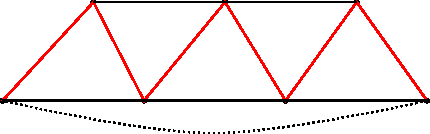
\includegraphics{./images/christofides}
\end{center}
\caption{A tight example for Christofides. MST in red, matching dotted. Edges have unit weight.}
\label{Fig:christofidesTight}
\end{figure}

For general TSP, without the triangle inequality, there is probably no $\alpha(n)$-approximation algorithm for any polynomial time computable function $\alpha$. That is, unless $P=NP$.

If we had such an approximation we could solve the hamiltonian circuit problem which is known to be NP-hard. In the hamiltonian circuit problem we don't have a complete graph like with TSP. We modify by setting all weights in $E$ to $1$ and add edges with weight $\alpha(n)\cdot n$ to obtain a complete graph.

Our assumed $\alpha(n)$ approximation would then solve the problem of finding the circuit. If a circuit exists there is a tour of cost $n$. If no circuit exists the cost of any tour is at least $\alpha(n)n$, because we need to take at least one of the expensive edges. An $\alpha(n)$ approximation can distinguish between these cases, so it can decide whether there is a circuit.

This type of reduction is called gap reduction.

\section{Knapsack}

The Knapsack problems asks to maximise the profit of a subset of items such that the weight of the set doesn't exceed some bound.

A classic approximation is to order the items by "profit density"

\[\frac{c_i}{w_i} \leq \frac{c_j}{w_j} \quad \forall i<j\]

We then take the best of

\[l = \max \{j\in \{1,\ldots, n\}| \sum w_j \leq K\} \qquad \{l+1\}\]

This is a 2-approximation. We can prove this by looking at the LP relaxation of the following ILP

\begin{align*}
\max \quad & \trans c s\\
s.t.\quad & \trans w s \leq K
	& s_i \in \{0,1\} && \forall i
\end{align*}

Obviously OPT$\geq z^*$ where $z^*$ is the optimal value of the relaxation. Since we also have

\[z^* \leq \sum_{j=1}^{k+1} c_j\]

Then we have

\[\max \{\sum_{j=1}^k c_j, c_{k+1}\} \geq \frac 12 \sum_{j=1}^{k+1} c_j \geq \frac 12 z^* \geq \frac 12 OPT\]

\marginpar{Lecture 22}
\section{LP-based approximation algorithms}

There are different approaches how to construct approximation algorithms from Linear Programs. Either we can find some suitable rounding scheme for a relaxed version of the LP or we use the LP as a bound in some other algorithm.

For the first approach the hard part is usually finding a suitable LP formulation s.t. it can be solved in polynomial time and we can deduce some error bounds when generating exact solutions from the relaxed LP constraints.

\subsection{Simple Rounding}

The naive approach to LP approximation is to just use the relaxed version of the ILP and round the answers to get an integral solution. Which rounding scheme can be used depends on the kind of constraints we have, not every rounding will produce feasible solutions in all cases.

We will study this technique using an example.

\begin{Ex}[Weighted Vertex Cover] We have a graph with weighted nodes. We want to find a miminum weight subset of vertices that covers every edge, i.e. every edge has at least one endpoint in the subset of nodes we chose.

One possible way to write that down as an LP is this:

\begin{align*}
\min \quad & \sum_{v\in V} x_v w_v\\
s.t. \quad & x_u+x_v \geq 1\\
	& x_v\in \{0,1\}
\end{align*}

We want $x_v$ to be $1$ iff the node is in our cover. Solving the relaxed version will give us some fractional solution. We round $x_v$ up, if it's larger than $\frac 12$, else we set it to zero.

This is a feasible integral solution, since we have for any edge $(u,v)$ that $x_v+x_u\geq 1$. So at least one of them has to be $\geq \frac 12$ hence we will round at least one value up to $1$.

This also gives us the approximation factor. It could happen that all $x_v$ are exactly $\frac 12$. We round them all up but the optimal solution may only need one of the vertices. Obviously we take twice the number of vertices in the worst case and thus this is a $2$-approximation.

In fact it seems that nobody knows a better algorithm. There is however a lower bound of $1.36$.

There is a nice structural insight about the polytope of this integral. We claim that it has vertices that are half-integral, i.e. $\in \{0,\frac 12,1\}$.

The proof isn't difficult. Assume we have some basic feasible solution $x$ that is not half integral. There has to be at least one value that is larger than $\frac 12$ and one that is smaller. Define the following sets

\[V_+ = \{v \in V | \frac 12 < x_v < 1\} \qquad V_- = \{v\in V |0 < x_v < \frac 12\}\]

We construct two new solutions from $x$ and those two sets. For $\epsilon > 0$

\[y_v = \begin{cases}
x_v + \epsilon & x_v \in V_+\\
x_v - \epsilon & x_v \in V_-\\
x_v & \text{otherwise}\end{cases} \qquad z_v = \begin{cases}
x_v - \epsilon & x_v \in V_+\\
x_v + \epsilon & x_v \in V_-\\
x_v & \text{otherwise}\end{cases}\]

By choosing $\epsilon$ small enough we can make sure that this remains feasible, i.e. $0<y_z <1$. Obviously $x$ is a convex combination of those. But if $x$ was optimal it was a vertex of the polyhedron and hence it can't be a combination of two other feasible points.

Note that this construction won't work for the $\frac 12$ case as we wouldn't get two different solutions

\end{Ex}

\subsection{Randomised Rounding}

We interpret the fractional values in the optimal solution as probabilities to set $x_j$ to $1$.

Since we use randomisation our approximation bounds will use the expected value (this slightly changes the previous definition).

\begin{Ex}[MAX SAT] We have a boolean formula in CNF with $m$ clauses and $n$ variables $v_j$. Each clause $C_i$ has a weight $w_i$ and we want to find an assignment of the variables such that the total weight of the satisfied clauses is maximised (note: we don't care about the truth value of the formula at all).

Let $W= \sum_{i=1}^m W_i $ be the random variable that indicates the total weight of the satisfied clauses in the solution of our algorithm.

The trivial algorithm sets every variable to true with probability $\frac 12$.

For this algorithm we have

\[\E(W_i) = \left(1-\frac{1}{2^{k(i)}}\right)w_i\]

where $k(i)$ is the number of literals in the clause. This is trivially right because a clause is satisfied if not all literals in the clause are set to false. So if we have $k(i)$ literals the probability to set them all to false is $1/2^{k(i)}$.

So for the expected outcome we have

\[\E(W) = \sum \E(W_i) = \sum_{i=1}^m \left(1-\frac{1}{2^{k(i)}}\right) w_i \geq \left(1-\frac{1}{2^{\bar k}}\right) \sum_{i=1}^m w_i\]

Where $\bar k$ is the minimal number of variables in any clause. So we have a 2-approximation

\[\left(1-\frac{1}{2^{\bar k}}\right) \sum_{i=1}^m w_i \geq \frac 12 \text{OPT}\]

But we can do better. 

Let $J^+(i)$ ($J^-(i)$) be the set of indices of non-negated (negated) variables in $C_i$. Consider the following LP

\begin{align*}
\max \quad & \sum_{i=1}^m w_iz_i\\
s.t. \quad &\sum_{j\in J^+(i)} y_i + \sum_{j\in J^-(i)} (1-y_i) \geq z_i && \forall i\\
&0\leq z_i, y_j \leq 1
\end{align*}

The idea is to use the variables $y_j$ for the boolean variables and the $z_i$ for the clauses. We need to make sure that a clause is only set to "satisfied" if at least one $y_j$ is set to true, if it is non-negated in the clause or false in the other case.

If we solve the LP and set $y_j$ to true with probability $y_j^{LP}$ we claim an approximation guarantee of 

\[\frac {e}{e-1} \approx 1.6\]

To prove that we need the following:

\[\E(W_i) \geq \left(1-\left(1-\frac{1}{k(i)}\right)^{k(i)}\right)w_iz_i^{LP}\]

w.l.o.g. all literal in $C_i$ appear in non-negated form and $C_i=(v_i \vee v_2 \vee \ldots \vee v_{k(i)})$. Then the probability that $C_i$ is satisfied is, as before:

\begin{align*}
1-P(\text{all lit. false}) &= 1- \prod_{i=1}^{k(i)} (1-y_j^{LP})\\
\intertext{We can bound that by using the AM-GM\footnote{Arithmetic mean vs. geometric mean} inequality}\\
	&\geq 1-\left(\frac {1}{k(i)}\sum_{i=1}^{k(i)} (1-y_j^{LP})\right)^{k(i)}\\
	&= 1-\left(1-\frac{1}{k(i)}\sum_{i=1}^{k(i)}y_j^{LP}\right)^{k(i)}\\
\intertext{From the constraint in the LP we can bound that sum}\\
	&\geq 1-\left(1-\frac{1}{k(i)}z_i^{LP}\right)^{k(i)}\\
\end{align*}

We looking at that thing we see that we can bound the concave function 

\[g(z) = 1-\left(1-\frac zk\right)^k\]

over the interval $[0,1]$ by a linear function 

\[f(z) = 1-\left(1-\frac 1k\right)^k z\]

Note that $f(0)=g(0)$ and $f(1)=g(1)$. Thus we get

\[1-\left(1-\frac{1}{k(i)}z_i^{LP}\right)^{k(i)} \geq \left(1-\left(1-\frac{1}{k(i)}\right)^{k(i)}\right)z_i^{LP}\]

And we have proven a bound on $\E(W_i)$. Then we can bound the expected value of the whole thing.

\begin{align*}
\E(W) &= \sum_{i=1}^W \E(W_i)\\
	&\geq \sum_{i=1}^W \left(1-\left(1-\frac{1}{k(i)}\right)^{k(i)}\right) z_i w_i\\
	&\stackrel{k\geq k(i)}{\geq} \sum_{i=1}^m \left(1-\left(1-\frac{1}{k}\right)^k\right) z_i^{LP}w_i\\
	&\geq (1-\frac 1e)\text{OPT}
\end{align*}
\end{Ex}

\marginpar{Lecture 23}
\section{The Cutting Stock Problem}
We're given $r$ rods of length $L$ and have a demand of $d_i$ pieces of length $l_i$. We want to cut the rods s.t. we meet the demand with a minimal number of raw rods.

Clearly

\[K:=\sum \frac{d_il_i}{L}\]

is a lower bound for the number of rods we need.

\subsection{Greedy Heuristic}

We will start with a greedy approach that guarantees a $2k+1$ approximation.

Initially all rods have the full length. In order to cut a piece we use an already used rod whenever possible, otherwise we start a new rod.

The analysis goes as follows: Let $G$ be the number of rods used by the algorithm. For each $i$ between $1$ and $G$ let $u_i$ be the used part and $w_i$ the waste. W.l.o.g. ordered decreasingly: $w_1\geq w_2\geq \ldots$. When we started to use the $j$th rod there wasn't enough room to use the $j-1$th. Thus $u_j\geq w_{j-1}$. We can write

\begin{align*}
G\cdot L &=  \sum_{j=1}^G (u_j+w_j)\\
	&= \sum_{j=1}^G u_j + \sum_{j=2}^G u_j +w_G\\
	&\leq L+2\sum_{j=1}^G u_j\\
	&\leq L + 2KL
\end{align*}

Thus $G\leq 2K+1$.

An alternative analysis distinguishes between "long" pieces that are longer than $L/2$ and "small" pieces. Assigning every long piece to a single rod assures that those are at least 50\% filled. We can aggregate small pieces on one rod until it is at least 50\% full, because small pieces are smaller than $L/2$. So in both cases we have a $2K+1$ approximation.

\subsection{Using an ILP}

We introduce variables $z_1,z_2,\ldots , z_t$, $t = \sum d_i$ s.t. 

\[z_j=\begin{cases} 1 & \text{rod j is used}\\
0 & \text{otherwise}\end{cases}\]

we also need variables $x_{ij}$ that indicate that we can fit $x_{ij}$ many pieces of length $l_i$ into the $j$th rod (if it is used).

Thus we get the ILP

\begin{align*}
\min \quad & \sum z_j\\
\text{s.t.} \quad & \sum x_{ij}l_i \leq Lz_j\\
	& \sum_{j} l_ix_{ij} \geq d_i && \forall i
	&x_{ij} \in \N, z_j \in \{0,1\}
\end{align*}

This isn't a particularly good formulation because it contains a lot of symmetry: there are many possibilities to use $k$ rods if we have to specify \emph{which} $k$ to use. Problems with many optimal solutions are hard to solve, in general.

Obviously the LP relaxation of this program has the trivial optimal value $K=\sum \frac{d_il_i}{L}$, as we are allowed to cut fractionally and can thus fill our rods optimally. The following assignment to the LP variables does just that:

\[z_j = \begin{cases}
1 & 1 \leq j \leq \lfloor K\rfloor \\
K-\lfloor K \rfloor & j=\lfloor K\rfloor +1\\
0 & \lfloor K \rfloor +1\end{cases}\qquad x_{ij} = \frac{d_i}{K}z_j\]

\subsection{Cutting Patterns}

But we can get a better approximation by a more sophisticated ILP.

\begin{Def}[Cutting pattern] A cutting pattern is a set of numbers $(a_1,\ldots,a_k)$ s.t. $a_i\in \N$ and $\sum a_il_i\leq L$ and the sum is maximal, i.e. there is no more room left for any $l_i$.\footnote{The book by Bertsimas doesn't make this restriction}
\end{Def}

Let $P$ be the set of all cutting patterns (this is a very large set). We introduce a variable $x_p$ for every $p\in P$ that indicates the number of patterns $p$ that we used.

This gives us the following ILP

\begin{align*}
\min \quad & \sum x_p\\
s.t. \quad & \sum a_{p_i}x_{p_i} \geq d_i && \forall i
\end{align*}

\begin{Ex} $L=7$, $l_1=2$ $l_2=3$

\[P=\{(3,0),(2,1),(0,2)\}\]

This gives us the ILP

\begin{align*}
\min \quad & x_1+x_2+x_3\\
s.t.\quad & 3x_1+2x_2+0x_3 \geq d_1\\
	&0x_1 + 1x_2+ 2x_3 \geq d_2
	&x\in \N
\end{align*}
\end{Ex}

There are different rounding strategies that produce integer solutions from the LP

\begin{itemize}
\item round up
\item round down and use the greedy heuristic to satisfy the demands
\item add cuts, e.g. Gomory cuts
\item branch and bound
\end{itemize}

But how do we solve the LP anyway? $P$ may be huge.

The idea is to start with a small number of patterns that guaranteees the existence of a solution, e.g. one cut per $l_i$. Let $P'\subset P$ be a set of patterns that is currently in use. We know the optimal LP solution for $P'$ and would like to know if it optimal for $P$. We can view the $P\backslash P'$ cuts to have non basic variables, i.e. they are 0. Now we can just use the normal stopping criterion of the simplex algorithm and check whether the reduced cost is $\geq 0$.

The reduced cost can be computed as usual. Let $y_i$ be the multiplier of the $i$th row, i.e. the value of the corresponding dual variable. Then the reduced cost is the column $p$ is eual to

\[1-\sum_{i=1}^k y_ia_i\]

($1$ because the cost for all patterns is $1$) and there is a variable of negative reduced cost iff there is a vector $a_1,\ldots,a_k$ such that the constraint $\trans a l_i \leq L$ and $\sum y_ia_i \geq 1$

We can find that vector by solving a knapsack problem. We want to grab some items with weight $a$, s.t. we don't exceed a bound $L$ and want to maximise the profit. 

Although knapsack is NP-complete it is usually simple to solve in practice. One can use a dynamic programming based approach.

\paragraph{Knapsack via Dynamic Programming} We have a table with columns from $0$ to $W$ and rows $1$ to $k$ where $W$ is the capacity and $k$ is the number of items. In cell $(i,j)$ we write the maximal value of a knapsack with capacity $j$ using only items $0,\ldots, i$. The first row is easy. Suppose we have solved the first couple of rows. Then we can compute a new cell by deciding whether we want to use item $i$ or not. 

\begin{align*}
A(1,z) &= \begin{cases} c_1 & z\geq w_1\\
0 & \text{otherwise}\end{cases}\\
A(i,z) &= \max (A(i-1,z), A(i-1,z-w_i)+c_i)
\end{align*}

The second term in the maximisation only exists if $z\geq w_i$.

If $W$ is reasonably small, filling the table is fast.
\end{document}
